\documentclass{article}

\usepackage{tikz}
\usetikzlibrary{shapes.geometric, arrows.meta, positioning}
\usepackage[margin=1in]{geometry}
\usepackage{parskip}

\tikzstyle{process} = [rectangle, rounded corners, minimum width=4cm, minimum height=1.4cm, text centered, text width=4cm, draw=black, fill=blue!10]
\tikzstyle{arrow} = [thick,->,>=stealth]


\usepackage{graphicx} % Required for inserting images
\usepackage{multicol}
\usepackage{listings}
\usepackage{amsmath}
\usepackage{algorithm}
\usepackage{algpseudocode}

\lstset{
  basicstyle=\ttfamily\small,
  breaklines=true,
  frame=single,
  columns=flexible,
  tabsize=2
}

%\usepackage[linesnumbered,ruled,vlined]{algorithm2e}
\usepackage{hyperref}
\usepackage{listings}
\usepackage[a4paper, margin=1.5in]{geometry}
\title{FYP_final_27}
\author{dev.banthia21 }
\date{April 2025}


\begin{document}


\section{Abstract}

This project presents an intelligent, hybrid data extraction pipeline for real estate documents, with a focus on property deeds. The solution combines a machine learning-based approach—leveraging a BERT-based Named Entity Recognition (NER) model to identify complex fields—with a rule-based pattern matching system for extracting regular, well-structured fields. OCR preprocessing is handled by Azure OCR, and the system outputs structured data in CSV/Excel format without uncertainty estimation. \\

Evaluation on a test dataset of 400 deed documents—spanning warranty deeds, special warranty deeds, statutory warrants, and warranty deeds with vendor liens—showed over 75\% field-level accuracy across 20 target fields. A field prediction was counted as correct when it had at least 80\% overlap with the ground truth. \\

The layered architecture balances the generalisation capability of transformer-based models with the precision and interpretability of deterministic rules. While currently a prototype, the system shows strong potential for deployment, with scalability considerations for processing over 10,000 documents per day. If successful, it is expected to reduce manual data entry effort by at least 30\% in a workflow currently involving over 200 personnel. \\

Future work involves extending this approach to additional document types such as mortgages and validating performance on larger datasets. This work lays the foundation for scalable, high-accuracy automation in legal document processing. \\

\section{Introduction}

\subsection{Business motivations}

In the real estate industry, structured property data plays a pivotal role in enabling accurate decision-making, efficient operations, and the development of competitive digital platforms. With the growing digitisation of property transactions, companies across the sector—including data aggregators, real estate marketplaces, investment firms, and regulatory bodies—are increasingly focused on automating the extraction of key information from legal documents such as deeds, mortgages, and foreclosure agreements. \\

The demand for this data stems from several critical business needs. For real estate marketplaces, structured data underpins advanced search functionality, personalised recommendations, and transparent listings. Accurate information about property ownership, pricing, and legal status enhances user trust and improves the overall customer experience. Investors and financial institutions rely on such data for risk assessment, portfolio management, and underwriting decisions. Meanwhile, data solutions providers require scalable pipelines to aggregate property data from diverse sources and jurisdictions into unified, queryable databases. \\

In addition to supporting commercial platforms and analytics, accurate property data extraction also plays a critical role in legal compliance and title indexing. Title indexing is the process of systematically cataloguing property records to establish a clear chain of ownership, identify liens or encumbrances, and ensure the legal validity of property transactions. \\

County recorders, legal firms, and title insurance companies rely on accurate indexing of deed documents to facilitate property transfers and protect against disputes or fraud. Automating the extraction of relevant fields such as grantor and grantee names, legal descriptions, and parcel identifiers is therefore essential not only for operational efficiency but also for maintaining compliance with legal standards in real estate documentation. \\

\subsection{Challenges in Automated Data Extraction from Real Estate Documents}

Automating the extraction of structured data from real estate documents presents several critical challenges, both in terms of data quality and operational feasibility. \\

A primary obstacle lies in the nature of the source files—most documents are scanned images with poor resolution, skew, and inconsistent formatting. Document layouts vary significantly across counties, time periods, and document types, making reliable text extraction difficult. However, this challenge is largely mitigated by modern deep learning-based OCR tools such as Azure OCR, which are capable of handling noisy, irregular scans at a relatively low cost \cite{azureocr}. \\

The second major challenge stems from the unstructured, legal nature of the content. Deeds and mortgages often contain domain-specific terminology, complex phrasing, and high variability in how key information is presented. This makes the consistent identification and extraction of fields like party names, addresses, or legal descriptions a non-trivial task. \\

With the advent of generative large language models (LLMs), it may seem natural to apply them to such problems. Indeed, LLMs demonstrate strong capabilities in understanding and summarising unstructured text. However, their use in high-volume legal data pipelines introduces serious concerns. Hallucination—the generation of text not present in the source—is an inherent risk, especially for long documents where key information may be scattered across multiple pages \cite{ji2023survey}. LLMs also struggle with retaining factual accuracy across large contexts, such as 20-page mortgage documents. \\

Moreover, the cost of deploying LLMs at scale is prohibitive. Whether accessed via commercial APIs or hosted in-house, their compute requirements and token-based pricing far exceed acceptable industry thresholds \cite{openai2024pricing}. For context, the standard processing budget for a mortgage document is approximately 0.2 cents. \cite{bpodataentry} Processing 10,000 multi-page documents daily using LLMs would significantly surpass this limit, making them unsuitable for core field extraction in production settings. \\

\subsection{Project Aim and Scope}

The primary aim of this project is to design an automated workflow capable of consistently achieving over 70\% accuracy in field identification across diverse types of real estate \textit{deeds}. The focus is strictly limited to deed documents; while similar in structure, \textit{mortgages} and other legal documents such as foreclosure records or invoices contain different fields and will require model retraining. However, the architecture and methodology developed here are intended to be extensible to these other document types once the pipeline demonstrates reliable performance on deeds. \\

The system is designed to extract the following fields from each deed:

\begin{multicols}{2}
\begin{itemize}
    \item Buyer name
    \item Seller name
    \item Buyer address
    \item Property address
    \item Assessor's parcel number
    \item Seller organization
    \item Buyer organization
    \item Recording date
    \item Document number
    \item Recording book number
    \item Recording page number
    \item Sales price amount
    \item Document date
    \item Signature date
    \item Effective date
    \item Document header
\end{itemize}
\end{multicols}

An annotated dataset of 7,700 deed documents is available for training and evaluation. However, this dataset includes ground truth labels for only the first seven fields. Due to the high cost and complexity of manual annotation, the remaining fields are to be captured using a \textit{rule-based pattern matching} approach. Once the rule-based extraction demonstrates high precision, its outputs can be used to generate pseudo-labeled data for training, effectively \textit{bootstrapping} the model to learn additional field types. \\

This approach offers a scalable and cost-efficient path forward, especially considering the anticipated daily volume of up to 10,000 documents. With continuous incoming data and iterative model retraining, the system is designed to improve over time and \textit{resist overfitting}, enabling it to generalise effectively to new layouts and unseen variations.

\subsection{Budget Constraints and Operational Impact}

Beyond the technical challenges, this project is shaped by stringent budgetary considerations. The current cost of processing each deed document is approximately \$0.10, amounting to an annual expenditure of nearly \$500,000 given the projected volume of over 10,000 documents per day. Relying solely on generative large language models (LLMs) for field extraction would far exceed this budget due to their high computational and token-based costs. Consequently, LLMs are excluded from the core extraction pipeline. \\

These financial constraints also influence the selection of OCR tools. It is essential to strike a balance between cost-efficiency and accuracy when choosing between commercial OCR services such as Azure OCR, Google Cloud Vision OCR, or potential open-source alternatives. \\

The potential impact of this project is significant. A successful implementation will not only improve operational efficiency by automating a labor-intensive process, but also enable the team to scale operations almost indefinitely. With in-house hardware resources as the only limiting factor, this workflow could support a major transformation in document processing capacity—positioning the organisation to win high-value clients and expand into new markets. \\

\section{Background}

\subsection{Real Estate Deeds: Structure and Content}

A real estate deed is a legal document used to transfer ownership of real property from one party to another. It is typically recorded by the county clerk or recorder's office and serves as the official, legally recognized evidence of a property transaction. The deed establishes who the grantor (seller) and grantee (buyer) are, and describes the property being transferred. \\

Deeds contain both essential and supplementary information. The essential fields generally include:
\begin{itemize}
\item Grantor (seller) name
\item Grantee (buyer) name
\item Property address
\item Legal description of the property
\item Assessor's Parcel Number (APN)
\item Recording date
\item Document number
\item Sales price (consideration amount), when applicable
\item Signatures and effective date
\item Party organizations (if applicable)
\end{itemize}

These fields are critical for indexing, title verification, and ensuring legal validity. Other content, such as boilerplate legal language, disclaimers, stamps, seals, and handwritten annotations, while legally necessary, is usually not relevant for structured data extraction. \\

This project involves deed documents sourced from dozens of counties across the United States. There is no standardized national format for deeds; even within a single county, formatting can vary depending on document age, software used, or recording procedures. \\

Format variations include:
\begin{itemize}
\item Field positioning: the same field may appear at different locations
\item Layout differences: single vs. multi-column, left-aligned vs. justified
\item Use of field labels: present in some documents, embedded in others
\item Variability in casing and punctuation
\item Presence or absence of structured sections or tables
\item Handwritten notes, stamps, and scanning artifacts
\end{itemize}

\subsection{Linguistic Variability and the Limitations of Rule-Based Extraction}

In addition to layout variability, deeds also exhibit significant linguistic variation. Important fields are often embedded within long, formal legal sentences using archaic language and inconsistent phrasing. This makes extraction using rigid rule-based methods unreliable. \cite{harriscountydeeds}

\textbf{Example 1: Grantee (Buyer) Name}
\begin{quote}
\textit{"...the said party of the first part does hereby grant, bargain, sell, and convey unto John Doe, of the County of Norfolk and State of Massachusetts, the premises described as follows..."}
\end{quote}

Here, the grantee's name appears without a clear label and is surrounded by verbose phrasing. Rule-based systems would need complex, fragile patterns to reliably extract such information.

\textbf{Example 2: Consideration Amount (Sales Price)}
\begin{quote}
\textit{"In consideration of the sum of One Hundred Forty-Five Thousand and 00/100 Dollars (\$145,000.00), the receipt whereof is hereby acknowledged..."}
\end{quote}

This example demonstrates mixed numeric and textual representations of the sales amount within a broader legal sentence.

\textbf{Example 3: Document Date}
\begin{quote}
\textit{"...witnesseth that this indenture was made the fourteenth day of June, in the year of our Lord two thousand and twenty..."}
\end{quote}

Such expressions are non-standard and require contextual understanding to convert into structured formats.

\textbf{Example 4: Parcel Number (APN)}
\begin{quote}
\textit{"...being the same premises identified on the municipal tax maps as Lot 17, Block 42, also known as Parcel No. 220-064-017..."}
\end{quote}

The field "Parcel No." is embedded within geographic and historical context, not presented as a labeled value.

Due to this level of variability, rule-based extraction methods are limited in their ability to generalize across unseen formats. They require extensive handcrafted rules, are brittle to minor deviations in language, and do not scale well.

Machine learning-based techniques offer a more robust alternative, particularly for extracting fields such as buyer and seller names and addresses, which exhibit a high degree of variation in phrasing and structure. By learning patterns from data rather than relying on fixed templates, ML-based models are better equipped to handle diverse expressions of the same information and adapt to new, unseen document formats.


\subsection{Model Architectures for Named Entity Recognition}

Named Entity Recognition (NER) is a token-level sequence labeling task. It requires the model to capture both local and global context, maintain consistency across labels, and generalize well to linguistic variations. This section traces the evolution of NER models—from early sequential neural networks to modern transformer-based architectures—highlighting how representations of words and context modeling have progressed in tandem.

\paragraph{Recurrent Neural Networks.}
Recurrent Neural Networks (RNNs) are designed to process sequential data by maintaining a hidden state that captures information from prior time steps. At each time step $t$, the hidden state $h_t$ is updated as:

\[
h_t = \tanh(W_{hh} h_{t-1} + W_{xh} x_t + b)
\]

where $x_t$ is the input vector, typically a \emph{word embedding}, and $W_{hh}, W_{xh}$ are learned weight matrices. This formulation allows RNNs to model dependencies in a sequence. However, their training is hindered by vanishing and exploding gradients \cite{bengio1994learning}, which make it difficult to capture long-range dependencies.

\paragraph{Word Embeddings: Motivation and Foundation}

To feed words into models like RNNs, we must first convert them into dense vector representations. One-hot encodings are sparse and fail to capture semantic similarity. Word embeddings address this by mapping each word $w_i$ to a continuous vector $\mathbf{e}_i \in \mathbb{R}^d$, such that similar words (e.g., \texttt{bank} and \texttt{money}) have closer representations.

\paragraph{Continuous Bag of Words Architecture}

The Continuous Bag of Words (CBOW) model, a precursor to neural sequence models, learns embeddings by predicting a target word from its surrounding context \cite{mikolov2013efficient}. Although effective in capturing word-level semantics, CBOW operates on bag-of-words assumptions—ignoring word order—and produces context-independent embeddings.

These embeddings were essential enablers for the next wave of models—sequential architectures that process word vectors in context-aware ways.

\paragraph{Long Short-Term Memory (LSTM).}
LSTM networks mitigate RNN limitations by introducing gating mechanisms that regulate information flow. Each LSTM cell maintains both a memory state $c_t$ and a hidden state $h_t$:

\begin{align*}
f_t &= \sigma(W_f x_t + U_f h_{t-1} + b_f) \quad \text{(forget gate)} \\
i_t &= \sigma(W_i x_t + U_i h_{t-1} + b_i) \quad \text{(input gate)} \\
o_t &= \sigma(W_o x_t + U_o h_{t-1} + b_o) \quad \text{(output gate)} \\
\tilde{c}_t &= \tanh(W_c x_t + U_c h_{t-1} + b_c) \quad \text{(candidate update)} \\
c_t &= f_t \odot c_{t-1} + i_t \odot \tilde{c}_t \\
h_t &= o_t \odot \tanh(c_t)
\end{align*}

The use of word embeddings as input enables LSTMs to leverage distributional semantics while learning temporal dependencies. However, traditional LSTMs only consider past context.

\paragraph{Bidirectional LSTMs.}
To incorporate both past and future context, Bidirectional LSTMs (BiLSTMs) \cite{huang2015bidirectional} process the sequence in forward and backward directions. For each token, the final representation is the concatenation of both hidden states:

\[
h_t = \text{concat}(\overrightarrow{h}_t, \overleftarrow{h}_t)
\]

This dual perspective is particularly useful in NER, where the meaning of a word often depends on its neighbors. BiLSTMs use pretrained word embeddings as input, allowing the model to benefit from both semantic priors and contextual dynamics.

\paragraph{BiLSTM-CRF Architecture.}
While BiLSTMs provide rich contextualized representations for each token, their output at each timestep is typically passed through a softmax classifier to predict the entity label independently. This approach ignores dependencies between labels, which are crucial in sequence labeling tasks like NER. \\

To address this, a Conditional Random Field (CRF) layer is often placed on top of the BiLSTM outputs \cite{lample2016neural}. The CRF considers the joint probability of the entire label sequence rather than making per-token decisions. This allows it to enforce valid label transitions and discourage implausible ones—such as assigning the tag sequence \texttt{[B-ORG, I-PER]} which violates BIO tagging conventions. \\

Formally, let $X = (x_1, x_2, \dots, x_n)$ be the input sequence and $Y = (y_1, y_2, \dots, y_n)$ the sequence of predicted labels. The BiLSTM outputs emission scores $s_t(y_t)$ for each token $t$, and the CRF defines a transition score $T_{y_{t-1}, y_t}$ between adjacent labels. The total score for a sequence is: \\

\[
\text{Score}(X, Y) = \sum_{t=1}^{n} \left( T_{y_{t-1}, y_t} + s_t(y_t) \right)
\]

During training, the CRF maximizes the log-probability of the correct label sequence by normalizing over all possible sequences:

\[
\log P(Y \mid X) = \text{Score}(X, Y) - \log \sum_{Y'} \exp(\text{Score}(X, Y'))
\]

At inference time, the most likely label sequence is decoded using the Viterbi algorithm. This combination—BiLSTM for context and CRF for structure—enables both fine-grained representation and global label coherence, making it especially effective in legal and structured document NER tasks. \\

\paragraph{Limitations of Recurrent Models.}
Despite their historical success, RNNs and LSTM-based models suffer from multiple limitations that hinder their scalability and effectiveness in industrial settings. \\

\textbf{1. Sequential Bottleneck.}
RNNs and LSTMs are inherently sequential: the hidden state at time $t$ depends on the computation of all previous timesteps. This dependency chain makes it impossible to parallelize token computations across a sequence. Even with optimized hardware like GPUs, this results in poor throughput and latency—especially problematic for long legal documents often encountered in OCR pipelines. \\

\textbf{2. Gradient Instability.}
While LSTMs alleviate the vanishing and exploding gradient problem through gating mechanisms and memory cells, they do not eliminate it entirely. As sequence length increases, gradients may still decay or amplify through multiple layers and timesteps, leading to unstable or ineffective learning \cite{pascanu2013difficulty}. This is particularly noticeable in very deep LSTM stacks or when processing long-range dependencies beyond a few hundred tokens. \\

\textbf{3. Limited Long-Range Modeling.}
Although BiLSTMs allow access to both past and future context, they struggle to model truly long-distance dependencies. The memory of earlier tokens fades as the sequence grows longer, and fixed-size hidden states limit the expressiveness of token representations over extended contexts. \\

\textbf{4. Static Context Windows.}
Even when bidirectional, LSTMs apply the same computation at every step, without dynamically weighting the importance of other tokens. This lack of adaptive attention prevents the model from focusing on highly relevant but distant words, a common need in entity extraction from dense legal language. \\

These limitations—combined with poor parallelism—motivated the shift toward transformer architectures, which offer a more scalable and flexible framework for learning contextual dependencies across entire sequences.



\paragraph{Transformers and Contextual Representations.}

Transformers \cite{vaswani2017attention} were introduced to overcome the key limitations of recurrent architectures—particularly their sequential processing bottleneck and difficulty modeling long-range dependencies. Rather than relying on recurrence, transformers employ a self-attention mechanism that enables each token in a sequence to directly attend to every other token, regardless of their position. This allows for efficient, parallelizable computation and rich global context modeling.

\vspace{2mm}
\noindent\textbf{Input Representation.}  
Let $x_1, x_2, \dots, x_n$ denote the input token sequence. Each token is mapped to a continuous embedding vector $\mathbf{e}_i \in \mathbb{R}^d$. However, since transformers are permutation-invariant by design, positional information must be explicitly injected. This is achieved by adding a positional encoding $\mathbf{p}_i$ to each embedding, forming the layer input:

\[
\mathbf{z}_i^{(0)} = \mathbf{e}_i + \mathbf{p}_i
\]

The positional encodings $\mathbf{p}_i$ can be either fixed (e.g., sinusoidal) or learned during training.

\vspace{2mm}
\noindent\textbf{Self-Attention Mechanism.}  
The core innovation of the transformer is its self-attention layer. Each input vector $\mathbf{z}_i$ is linearly transformed into three components:

\[
\mathbf{q}_i = \mathbf{z}_i W^Q, \quad \mathbf{k}_i = \mathbf{z}_i W^K, \quad \mathbf{v}_i = \mathbf{z}_i W^V
\]

where $W^Q, W^K, W^V \in \mathbb{R}^{d \times d_k}$ are learned projection matrices. These define:
\begin{itemize}
    \item \textbf{Query} $\mathbf{q}_i$: what the token seeks from others,
    \item \textbf{Key} $\mathbf{k}_j$: how relevant another token is,
    \item \textbf{Value} $\mathbf{v}_j$: the content to contribute if deemed relevant.
\end{itemize}

The relevance between tokens $i$ and $j$ is quantified by their scaled dot-product:

\[
\alpha_{ij} = \frac{\exp\left(\frac{\mathbf{q}_i^\top \mathbf{k}_j}{\sqrt{d_k}}\right)}{\sum_{j'=1}^{n} \exp\left(\frac{\mathbf{q}_i^\top \mathbf{k}_{j'}}{\sqrt{d_k}}\right)}
\]

The output for position $i$ is then a weighted sum over all value vectors:

\[
\text{Attention}(\mathbf{q}_i, K, V) = \sum_{j=1}^{n} \alpha_{ij} \mathbf{v}_j
\]

Or compactly, in matrix form:

\[
\text{Attention}(Q, K, V) = \text{softmax}\left( \frac{QK^\top}{\sqrt{d_k}} \right)V
\]

\vspace{2mm}
\noindent\textbf{Layer Composition and Contextualization.}  
Each transformer encoder layer comprises:
\begin{enumerate}
    \item \textbf{Multi-head self-attention:} Multiple parallel attention heads learn different contextual subspaces.
    \item \textbf{Feed-forward network (FFN):} A position-wise dense network applies non-linearity and transformation independently at each token.
\end{enumerate}

Residual connections and layer normalization are applied after both subcomponents to stabilize training:

\[
\text{LayerNorm}(X + \text{Attention}(X)) \rightarrow \text{LayerNorm}(X + \text{FFN}(X))
\]

By stacking $L$ such encoder blocks, each token representation becomes deeply contextualized—encoding not only its identity but its role within the full sentence.

\vspace{3mm}
\noindent\textbf{Advantages over RNNs.}  
Transformers offer several advantages compared to recurrent models:

\begin{itemize}
    \item \textbf{Parallelism:} Unlike RNNs/LSTMs, which must process tokens sequentially, transformers compute all token representations in parallel.
    \item \textbf{Global Dependency Modeling:} Self-attention allows any token to directly attend to any other, enabling effective modeling of long-range dependencies.
    \item \textbf{Gradient Stability:} Transformers avoid the vanishing/exploding gradient problem inherent in long unrolled RNNs, supporting deeper networks.
\end{itemize}

These properties make transformers highly scalable and well-suited for modern hardware acceleration.

\vspace{3mm}
\paragraph{Choosing BERT for NER.}

Among transformer-based models, we adopt BERT (Bidirectional Encoder Representations from Transformers) \cite{devlin2018bert}, which is pre-trained on large unlabeled corpora using two self-supervised objectives:

\begin{itemize}
    \item \textbf{Masked Language Modeling (MLM):} Randomly masks 15\% of tokens in each sequence and trains the model to predict them from context, encouraging deep bidirectional understanding.
    \item \textbf{Next Sentence Prediction (NSP):} Predicts whether two input sentences follow each other in the corpus, helping the model learn inter-sentence relationships.
\end{itemize}

BERT’s defining feature is its \emph{bidirectional self-attention}, which allows it to condition on both the left and right context when encoding any token. For example, in the sentence:

\begin{quote}
    \textit{"Jordan gave a lecture on Middle Eastern politics."}
\end{quote}

the word \textit{"Jordan"} can refer to either a person or a country. BERT uses the surrounding phrase \textit{"Middle Eastern politics"} to disambiguate it as a geopolitical entity—something unidirectional models like GPT cannot do during encoding.

\vspace{3mm}
\noindent\textbf{Context Window of BERT and Justification for Use.}  
Despite its strengths, BERT has a maximum input sequence length of 512 tokens. This limitation arises from the \textbf{quadratic time and memory complexity} of self-attention: for a sequence of length $n$, attention involves computing an $n \times n$ similarity matrix.

\begin{itemize}
    \item BERT-base (512 tokens): $512^2 = 262{,}144$ pairwise comparisons per layer.
    \item Longformer (4096 tokens): $4096^2 = 16{,}777{,}216$ comparisons—over 60x more.
\end{itemize}

While extended-context models like Longformer \cite{beltagy2020longformer} and BigBird \cite{zaheer2020bigbird} address this with sparse attention, they add architectural complexity and may incur slower inference. In our domain, such extended contexts are not strictly necessary—key fields like party names, parcel numbers, or legal descriptions tend to appear in concentrated spans.

Thus, BERT provides an optimal balance between contextual power, inference efficiency, and implementation simplicity. Its strong empirical performance, robust pretraining, and extensive ecosystem support make it the most pragmatic choice for our named entity recognition pipeline on real estate documents.



\subsection{Limitations of Using BERT Alone}

While transformer-based models such as BERT have demonstrated strong performance in named entity recognition (NER) tasks involving person names, organizations, and addresses, they are not inherently well-suited for extracting structured or numeric data fields. This is particularly relevant in the context of deed documents, which contain key fields like document numbers, book and page numbers, and various date formats. \\

\textbf{1. Lack of pretraining on numeric patterns:} BERT is pretrained on large, general-purpose corpora such as Wikipedia and BookCorpus. These datasets are rich in natural language but sparse in structured numerical expressions. As a result, BERT does not natively learn how to handle patterns such as ``2021-048293'' or ``Book 8472, Page 392''. \\

\textbf{2. Tokenisation issues:} BERT's WordPiece tokenizer tends to split numeric tokens into multiple subword units. \cite{schuster2012japanese} For example, a document number like ``2021-048293'' may be tokenized into segments such as ``2021'', ``-``, ``048'', and ``293'', breaking up the semantic unity of the field and introducing noise during classification. \\

\textbf{3. No inductive bias for numeric structures:} Unlike rule-based systems, BERT has no built-in understanding that patterns like ``Book No. 8472'' or ``Parcel ID 220-064-017'' belong to a specific field type. It treats these tokens like any other arbitrary text, unless it has seen enough similar examples during fine-tuning. \cite{wallace2019nlpnumber} \\

\textbf{4. Attention dilution in long sentences:} In lengthy legal sentences, short numeric spans may receive disproportionately low attention weights. Without explicit positional guidance or layout cues, BERT may fail to assign sufficient importance to these spans. \\

\textbf{Implication:} For reliably extracting highly structured numeric fields, BERT alone may be insufficient. A hybrid approach that combines BERT-based entity recognition for unstructured fields with rule-based post-processing for deterministic patterns (e.g., dates, document numbers) offers a more robust and interpretable solution for end-to-end deed parsing.

\subsection{Regular Expressions for Field Extraction}

Regular expressions (regex) are a foundational tool for pattern matching, used to identify specific sequences of characters within text. \cite{friedl2006regex} In the context of field extraction from deed documents, regex facilitates the identification of structured tokens such as document numbers, dates, and parcel identifiers based on predefined textual patterns. \\

Regex enables the construction of both primitive and compound expressions. Primitive patterns match basic components—for example, \textbackslash d+ matches one or more digits, [-/] matches common separators, and \textbackslash b denotes word boundaries. These can be composed into more complex expressions to capture specific formats. For instance, a document number like "2021-048293" can be matched using \textbackslash d{4}-\textbackslash d{6}, while dates such as "06/14/2021" or "June 14, 2021" can be captured with tailored alternatives. \\

Regex is particularly effective when fields adhere to consistent structural rules, even within noisy or unstructured documents. It is computationally lightweight and easy to implement, making it a practical first-pass method for extracting well-defined numeric identifiers and standardized field types. \\

However, regular expressions have notable limitations. They are inherently brittle, requiring exact pattern matches, which makes them prone to failure when faced with inconsistent phrasing, formatting artifacts, or embedded legal language. Furthermore, regex lacks semantic understanding—it cannot infer meaning from context, which is critical when extracting ambiguous entities such as names or addresses that may vary in structure and location. Consequently, regex is best employed as a complementary technique within hybrid extraction systems, supporting more robust machine learning-based models that can generalize across variability.

\subsection{Hybrid Approach: Combining Regex and BERT for Field Extraction}

Given the diversity and complexity of real estate deed documents, a hybrid field extraction strategy is adopted that combines regular expressions for structured numeric fields with BERT-based models for context-dependent, variable text fields. This approach balances precision and flexibility, leveraging the strengths of both methodologies. \\

Regular expressions are used to extract fields that follow well-defined syntactic patterns, such as dates, document numbers, book/page references, and sales amounts. These patterns are carefully designed to account for a wide range of format variations observed across counties and document types. While regex is rigid and requires manual tuning, its reliability in identifying numeric fields with consistent delimiters makes it an effective tool for high-precision extraction. \\

In contrast, fields such as buyer and seller names, addresses, and legal entities are too variable in structure to be captured accurately by rule-based methods alone. For these fields, we employ a fine-tuned BERT-based model trained on annotated deed data. Unlike regex, BERT learns patterns from labelled examples and generalizes beyond seen formats. This is crucial when dealing with the linguistic variability and legal phrasing common in unstructured documents. \\

A key conceptual advantage of this hybrid setup is that regex-based extraction acts as an automatic annotator. Since thousands of deeds are processed daily, the successful pattern matching of numeric fields creates a growing pool of weakly labelled training data. This continuous stream of data can be used to retrain or fine-tune the BERT model on other fields, enabling the system to adapt and improve over time without full manual annotation. \\

While BERT may not excel at extracting exact numeric values, it often correctly identifies the surrounding context, helping localize the field of interest. In such cases, regex and BERT can be used in tandem—BERT handles the identification, while regex validates and extracts the precise value. This cooperative use of both tools enhances both robustness and accuracy, particularly in production environments where document variability is high and throughput requirements are large. \\

\section{Design}

We begin by presenting two high-level flowcharts that capture the core structure of our system. These diagrams serve as a conceptual overview to illustrate how different modules interact and fit together. All steps are explained in depth in the subsequent Implementation chapter. \\

The first flowchart outlines the one-time model training process, which prepares the transformer-based Named Entity Recognition (NER) model using annotated training data. Although training may be repeated for fine-tuning or retraining on new datasets, it is not part of the routine inference cycle. \\

The second flowchart depicts the full inference pipeline. This is the central operational component of the system and is executed for each new document. It leverages most of the dataset construction pipeline but omits training and focuses on text extraction, entity prediction, and post-processing. \\


The figure below outlines the complete preprocessing and training workflow for our Named Entity Recognition (NER) model. It begins with annotated data ingestion and ends with the training loop. Each stage is designed to ensure label consistency, contextual tokenization, and compatibility with transformer-based architectures.


\begin{center}
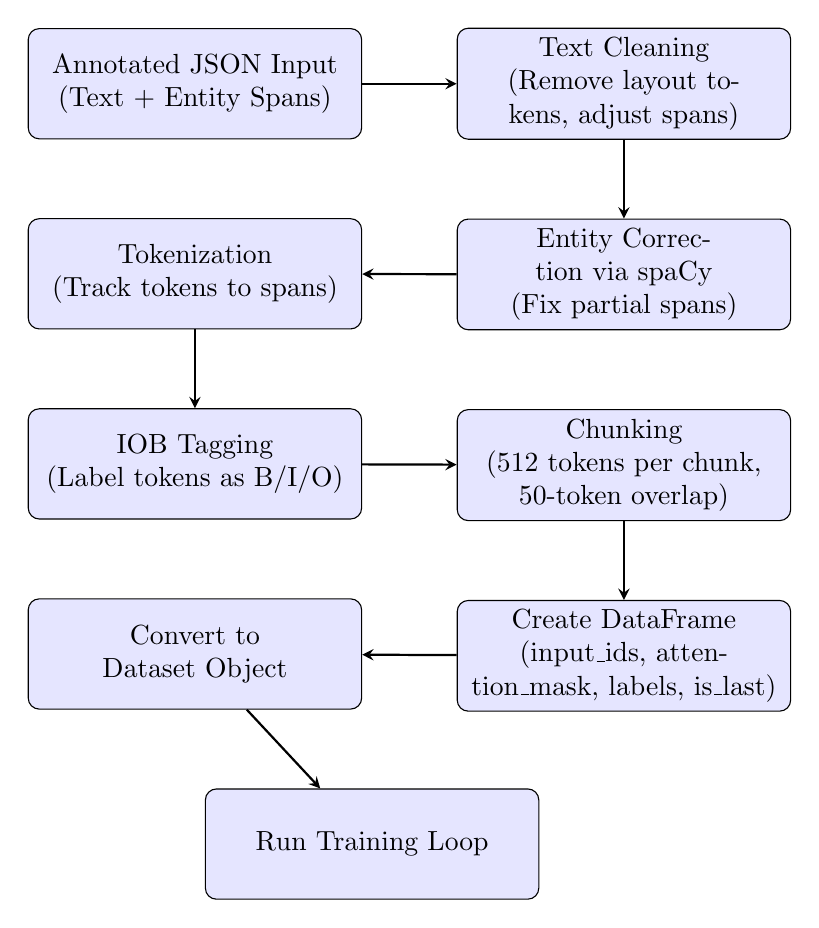
\begin{tikzpicture}[node distance=1cm and 1.2cm]
% Row 1
\node (json) [process] {Annotated JSON Input \\ (Text + Entity Spans)};
\node (clean) [process, right=of json] {Text Cleaning \\ (Remove layout tokens, adjust spans)};
% Row 2
\node (spacy) [process, below=of clean] {Entity Correction via spaCy \\ (Fix partial spans)};
\node (tokenise) [process, below=of json] {Tokenization \\ (Track tokens to spans)};
% Row 3
\node (iob) [process, below=of tokenise] {IOB Tagging \\ (Label tokens as B/I/O)};
\node (chunk) [process, below=of spacy] {Chunking \\ (512 tokens per chunk, 50-token overlap)};
% Row 4
\node (df) [process, below=of chunk] {Create DataFrame \\ (input\_ids, attention\_mask, labels, is\_last)};
\node (dataset) [process, below=of iob] {Convert to Dataset Object};
% Row 5
\node (train) [process, below=of dataset, xshift=2.25cm] {Run Training Loop};

% Arrows
\draw [arrow] (json) -- (clean);
\draw [arrow] (clean) -- (spacy);
\draw [arrow] (spacy) -- (tokenise);
\draw [arrow] (tokenise) -- (iob);
\draw [arrow] (iob) -- (chunk);
\draw [arrow] (chunk) -- (df);
\draw [arrow] (df) -- (dataset);
\draw [arrow] (dataset) -- (train);
\end{tikzpicture}
\end{center}

\paragraph{Step-by-Step Breakdown:}
\begin{itemize}
    \item \textbf{Annotated JSON Input:} Contains the full document text along with named entity spans.
    \item \textbf{Text Cleaning:} Removes layout artifacts and updates entity span indices accordingly.
    \item \textbf{Entity Correction via spaCy:} Uses heuristics to expand or fix annotation boundaries when partial matches are detected.
    \item \textbf{Tokenization:} Breaks down the cleaned text into subword tokens, mapping original entity spans to token indices.
    \item \textbf{IOB Tagging:} Assigns token-level labels following the standard Inside–Outside–Beginning (IOB) scheme.
    \item \textbf{Chunking:} Splits tokenized sequences into 512-token segments with a 50-token overlap to preserve context.
    \item \textbf{DataFrame Creation:} Stores token features such as input IDs, attention masks, token labels, and a document-end indicator.
    \item \textbf{Dataset Conversion:} Converts the DataFrame into a dataset object suitable for batching and training.
    \item \textbf{Training Loop:} Executes the fine-tuning of a transformer-based model using the prepared dataset.
\end{itemize}

\section*{Full Inference Pipeline}

\begin{quote}
\emph{This flowchart provides a high-level overview of the end-to-end inference pipeline. Each step is explained in further technical detail within the Implementation chapter.}
\end{quote}



\begin{center}
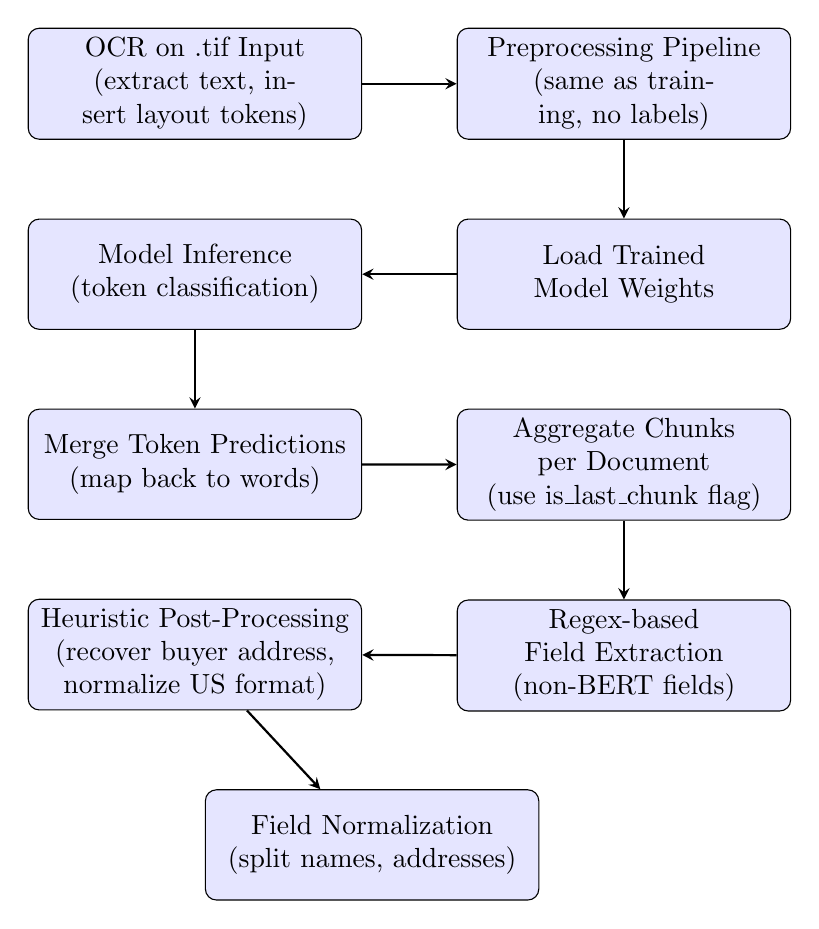
\begin{tikzpicture}[node distance=1cm and 1.2cm]
% Row 1
\node (ocr) [process] {OCR on .tif Input \\ (extract text, insert layout tokens)};
\node (prep) [process, right=of ocr] {Preprocessing Pipeline \\ (same as training, no labels)};
% Row 2
\node (loadmodel) [process, below=of prep] {Load Trained Model Weights};
\node (inference) [process, below=of ocr] {Model Inference \\ (token classification)};
% Row 3
\node (merge) [process, below=of inference] {Merge Token Predictions \\ (map back to words)};
\node (aggregate) [process, below=of loadmodel] {Aggregate Chunks per Document \\ (use is\_last\_chunk flag)};
% Row 4
\node (regex) [process, below=of aggregate] {Regex-based Field Extraction \\ (non-BERT fields)};
\node (heuristics) [process, below=of merge] {Heuristic Post-Processing \\ (recover buyer address, normalize US format)};
% Row 5
\node (final) [process, below=of heuristics, xshift=2.25cm] {Field Normalization \\ (split names, addresses)};

% Arrows
\draw [arrow] (ocr) -- (prep);
\draw [arrow] (prep) -- (loadmodel);
\draw [arrow] (loadmodel) -- (inference);
\draw [arrow] (inference) -- (merge);
\draw [arrow] (merge) -- (aggregate);
\draw [arrow] (aggregate) -- (regex);
\draw [arrow] (regex) -- (heuristics);
\draw [arrow] (heuristics) -- (final);
\end{tikzpicture}
\end{center}

\paragraph{Step-by-Step Breakdown:}
\begin{itemize}
    \item \textbf{OCR on .tif Input:} Runs optical character recognition on scanned images and injects layout tokens to preserve document structure.
    \item \textbf{Preprocessing Pipeline:} Applies the same steps as in training (cleaning, tokenization, chunking), but omits label generation.
    \item \textbf{Load Trained Model Weights:} Loads the pre-trained transformer model from saved checkpoint files for inference.
    \item \textbf{Model Inference:} Feeds tokenized chunks into the model to obtain predicted entity labels.
    \item \textbf{Merge Token Predictions:} Reconstructs full words from token predictions and maps token IDs back to text.
    \item \textbf{Aggregate Chunks per Document:} Uses the \texttt{is\_last\_chunk} flag to concatenate predictions across document chunks.
    \item \textbf{Regex-based Field Extraction:} Extracts structured fields not covered by BERT using pattern-based rules.
    \item \textbf{Heuristic Post-Processing:} Applies logic to fill missing fields (e.g., buyer address recovery), and standardizes US address formats.
    \item \textbf{Field Normalization:} Breaks composite fields like names and addresses into subcomponents (e.g., first, middle, last names; city, state, ZIP).
\end{itemize}


\section{Implementation}


\subsection{Fine-Tuning BERT for Named Entity Recognition}

To perform token-level field extraction from deed documents, we fine-tune BERT on a \emph{Named Entity Recognition} (NER) task. BERT's bidirectional transformer layers produce contextual embeddings for each input token, which are then classified into entity categories using a task-specific classification head.

\subsubsection{WordPiece Tokenization}

BERT uses a subword tokenization scheme known as \emph{WordPiece}. Instead of assigning embeddings to entire words, WordPiece breaks rare or unknown words into smaller units. For example:

\begin{center}
    \texttt{unaffordable} $\rightarrow$ [\texttt{un}, \texttt{\#\#afford}, \texttt{\#\#able}]
\end{center}

This allows the model to handle out-of-vocabulary words more gracefully. However, it also introduces a challenge for NER: entity labels are defined at the word level, while the input is tokenized at the subword level. To resolve this, labels are aligned only to the \emph{first subword} of each token. Subsequent subtokens are either ignored during loss computation or assigned a special label such as \texttt{X}.

\subsubsection{Entity Tagging Schemes}

We adopt the IOB tagging format \cite{ramshaw1995text} to annotate entities:
\begin{itemize}
    \item \texttt{B-FIELD}: Beginning of a field (e.g., \texttt{B-BUYER\_NAME})
    \item \texttt{I-FIELD}: Inside a field span
    \item \texttt{O}: Outside any entity
\end{itemize}

Alternatively, more expressive schemes like BILOU (Begin, Inside, Last, Outside, Unit) \cite{ratinov2009design} can be used to better capture field boundaries, but IOB remains standard in many NER datasets and is compatible with BERT’s token-level classification setup.

\subsubsection{Token Classification Layer}

Let $\mathbf{h}_i \in \mathbb{R}^d$ be the contextual embedding of token $i$ output by BERT's final layer. This is passed through a linear classifier:

\[
\mathbf{y}_i = \text{softmax}(\mathbf{W} \mathbf{h}_i + \mathbf{b})
\]

where $\mathbf{W} \in \mathbb{R}^{C \times d}$ and $\mathbf{b} \in \mathbb{R}^C$, with $C$ being the number of entity classes (e.g., \texttt{B-BUYER\_NAME}, \texttt{I-BUYER\_NAME}, \texttt{O}, etc.). The predicted probability distribution over labels is compared against the ground truth labels using the **cross-entropy loss**:

\[
\mathcal{L}_{\text{NER}} = -\sum_{i=1}^{n} \sum_{c=1}^{C} y_{i,c}^{\text{true}} \log(y_{i,c}^{\text{pred}})
\]

During training, gradients are backpropagated \cite{rumelhart1986learning} through both the classification head and BERT encoder layers, updating all parameters via gradient descent. This fine-tuning allows the model to adapt its general linguistic knowledge to the domain-specific patterns in real estate documents.

\subsubsection{Training Setup}

The model is fine-tuned on a labelled dataset of 7,700 deed documents. The input is preprocessed into token-label pairs, and training is performed using the Adam optimizer with a learning rate warm-up schedule. Common hyperparameters include:
\begin{itemize}
    \item Batch size: 16 or 32
    \item Learning rate: $2 \times 10^{-5}$ to $5 \times 10^{-5}$
    \item Epochs: 3–5
    \item Max sequence length: typically 512 tokens
\end{itemize}

\subsubsection{Inference and Output Mapping}

At inference time, each token receives a predicted label. Subword labels are mapped back to words using a label aggregation strategy (e.g., taking the label of the first subtoken). Consecutive spans with \texttt{B-}/\texttt{I-} tags are grouped into field-level predictions and postprocessed into structured outputs.

Field-level accuracy is measured using an overlap criterion—typically, a prediction is considered correct if it matches the ground truth with at least 80\% character-level overlap.

\begin{lstlisting}[caption={End-to-End Structured Entity Extraction Pipeline}, label={lst:end_to_end_pipeline}, language=Python, frame=single]
# Pseudocode for structured entity extraction pipeline

Initialize empty predictions_df  # This will store final structured predictions
Initialize empty list to accumulate document-level predictions

for each row in df:
    Extract token-level predictions and input IDs for the current chunk

    # Convert predicted label indices to human-readable entity tags
    mapped_labels = map(reverse_entity_mapping, raw_predictions)

    # Identify entity spans using label boundaries (BIO tagging scheme)
    # This function detects where a new entity starts and builds binary masks
    # indicating the token positions that form each entity
    entity_masks, entity_names = find_entities_in_text(mapped_labels)

    # Reconstruct original entity strings from token IDs using binary masks
    # For each mask, select the corresponding tokens, convert them to strings,
    # and merge subword tokens (e.g., "New", "##ark" → "Newark")
    entity_texts = show_sample(input_ids, entity_masks, entity_names)

    for each (entity_type, entity_text) in entity_texts:
        Append (entity_type, entity_text) to document-level predictions

    # Once the final chunk of the document is reached,
    # aggregate all extracted entity spans for the full document
    if current chunk is last:
        aggregated = aggregate_predictions(document-level predictions)
        Create new row with image/document name and aggregated fields
        Append row to predictions_df
        Reset document-level predictions

# Merge structured predictions with auxiliary metadata (e.g., recording details)
predictions_df = predictions_df.merge(recording_details_df, on="filename")

# Export or print results per document
for each row in predictions_df:
    Print document name and associated field-value pairs
\end{lstlisting}


\subsection{Labelled Dataset Format and Entity Alignment Pipeline}

To fine-tune the BERT-based Named Entity Recognition (NER) model for field extraction from deed documents, a robust multi-stage preprocessing pipeline was developed. The input consisted of raw OCR text and manually annotated character-level spans in a JSON format. This pipeline transformed the noisy, span-based annotations into a structure compatible with BERT’s token classification framework, ensuring that each token could be reliably assigned a label during training.

\subsubsection{Annotation Format}

Each record in the labelled dataset was stored as a JSON object containing:
\begin{itemize}
    \item \texttt{classes}: a list of field types such as \texttt{``BUYER NAME''}, \texttt{``SELLER NAME''}, \texttt{``PROPERTY ADDRESS''}, etc.
    \item \texttt{annotations}: a list of pairs \texttt{[text, \{entities\}]}, where \texttt{text} is the full OCR-extracted document and \texttt{entities} is a list of character-level spans in the form \texttt{[start\_char, end\_char, label]}.
\end{itemize}

For example:
\begin{verbatim}
["...unto John Doe, of the County...", {"entities": [[7, 15, "BUYER NAME"]]}]
\end{verbatim}

\subsubsection{Entity Cleaning and Boundary Correction}

Due to OCR artifacts, inconsistent annotation, and extraneous tokens, the following cleaning steps were applied:
\begin{itemize}
    \item Label typos (e.g., \texttt{``BUYER ADDDRESS''}) were normalized to standard forms.
    \item Only a curated set of core field types was retained.
    \item Artificial tokens such as \verb|<laysep@@##$$>| and escaped Unicode sequences (e.g., \verb|\u00a9|) were removed using regular expressions.
\end{itemize}

Cleaning altered the text content and could misalign character offsets. To fix this, entity positions were recalculated by computing the character count difference between the original and cleaned text up to each entity's start index. This offset correction preserved alignment between entity spans and the new cleaned text.

\subsubsection{Token Boundary Enforcement}

Even after cleaning, entity spans might not align with token boundaries. This misalignment arises because:
\begin{itemize}
    \item Entity start and end indices were manually annotated at the character level, independent of how BERT tokenizes text.
    \item BERT (and most NLP models) require entity spans to match token boundaries for correct label assignment.
\end{itemize}

To address this, the following procedure was used:
\begin{itemize}
    \item Tokens in the text were identified using regular expressions and stored as spans.
    \item Each entity span was checked for partial overlap with token boundaries.
    \item If a span intersected one or more tokens without fully covering them, its start and/or end indices were adjusted to snap to the nearest token boundary.
    \item If the resulting span was invalid (i.e., \texttt{start} $\geq$ \texttt{end}), it was discarded.
\end{itemize}

This clipping strategy reduced label noise caused by partially included tokens, which could otherwise confuse the model.

\subsubsection{Conversion to SpaCy-Compatible Format}

To ensure that annotated entity spans align correctly with token boundaries, each cleaned document was processed using \texttt{spaCy}, a widely used open-source natural language processing (NLP) library that provides efficient tokenization and linguistic annotations \cite{spacy}. \\

In \texttt{spaCy}, a processed document is represented by a \texttt{Doc} object. This object contains the original text along with tokenization metadata such as token indices and their corresponding character-level start and end positions. By converting each raw text string into a \texttt{Doc} object using \texttt{nlp.make\_doc(text)}, the pipeline gains access to this token structure, which is critical for aligning annotated character spans with tokens. \\

Each manually annotated entity span \texttt{[start, end, label]} was then passed to the method \texttt{doc.char\_span(...)}. This method attempts to convert a character-level span into a \texttt{Span} object, which represents a continuous sequence of tokens in the document. Importantly, \texttt{char\_span} includes an optional argument \texttt{alignment\_mode}, which determines how to handle spans that do not perfectly align with token boundaries. \\

In this pipeline, the mode \texttt{alignment\_mode="expand"} was used to address a common issue: annotated spans derived from OCR or human labelling often do not begin and end exactly at token boundaries. For example, a span might begin in the middle of a token (e.g., character 1 of the token ``John'') and end in the middle of another. If such a span were used directly during training, it would create ambiguity during token classification, as the model would not be able to cleanly assign a label to any individual token. \\

The \texttt{"expand"} mode resolves this by stretching the character span outward to the nearest full tokens. This ensures that entity spans are aligned cleanly with spaCy’s tokenization and are therefore compatible with token-level classification in transformer-based models. If a span could not be resolved to valid tokens even after expansion—such as if it landed entirely within whitespace or formatting artifacts—it was discarded to avoid injecting noise into the training set. \\

By leveraging spaCy’s alignment functionality in this way, the pipeline robustly transformed noisy, potentially misaligned entity annotations into token-aligned spans. This step was essential to bridge the gap between raw OCR-derived annotations and the requirements of models like BERT, which expect input labels to be defined at the token level.


\begin{lstlisting}[language=Python, caption=Entity Alignment and Cleaning Pipeline (Pseudocode)]
# Input: Annotated dataset D = [(text, entities)], Regex patterns P = [p1, p2, ...]
# Output: Cleaned and aligned dataset D'

for (text, entities) in D:

    # Step 1: Adjust entity boundaries based on pattern overlaps
    matches = find_all_regex_matches(text, P)

    updated_entities = []
    for (start, end, label) in entities:
        overlapping = find_overlaps((start, end), matches)

        for match in overlapping:
            if match partially overlaps (start, end):
                adjust entity boundaries to exclude match

        if start < end:
            updated_entities.append((start, end, label))

    # Step 2: Remove patterns globally and adjust entity offsets
    cleaned_text = remove_patterns(text, P)

    for (start, end, label) in updated_entities:
        offset = compute_offset_due_to_removed_patterns(text, cleaned_text, start)
        adjust entity start/end by subtracting offset

    # Step 3: Align entities with spaCy Doc
    doc = nlp.make_doc(cleaned_text)

    final_entities = []
    for (start, end, label) in updated_entities:
        span = doc.char_span(start, end, label=label)
        if span is valid:
            final_entities.append((span.start_char, span.end_char, label))

    D'.append((cleaned_text, final_entities))

return D'
\end{lstlisting}


\subsubsection{BERT Token Alignment and BIO Tagging}

After entity spans were aligned with token boundaries, the dataset was tokenized using HuggingFace’s \texttt{bert-base-uncased} tokenizer. Each document was passed through the tokenizer with the \texttt{return\_offsets\_mapping=True} argument, which returned both token identifiers and their corresponding character-level positions: \\

\begin{verbatim}
tokenizer(text, return_offsets_mapping=True)
\end{verbatim}

This produced:
\begin{itemize}
    \item \texttt{input\_ids}: a sequence of integer identifiers corresponding to subword tokens in BERT’s vocabulary.
    \item \texttt{offset\_mapping}: a list of \texttt{(start, end)} character positions indicating which part of the raw text each token corresponds to.
\end{itemize}

Each token was then assigned a label using the BIO (Begin–Inside–Outside) tagging scheme:
\begin{itemize}
    \item \texttt{B-FIELD}: indicates the beginning of an entity of type \texttt{FIELD}.
    \item \texttt{I-FIELD}: indicates that the token is inside (but not at the start of) an entity of type \texttt{FIELD}.
    \item \texttt{O}: indicates that the token does not belong to any entity.
\end{itemize}

The use of BIO tagging, rather than a simpler Inside–Outside (IO) scheme, is necessary to disambiguate adjacent entities of the same type. Without a \texttt{B-} tag, sequences like \texttt{I-BUYER NAME, I-BUYER NAME} could either mean a single multi-token entity or two consecutive entities of the same type, making decoding ambiguous. The BIO scheme resolves this by explicitly marking the boundary where a new entity begins. \\

While more expressive schemes such as BILOU (Begin, Inside, Last, Outside, Unit) offer finer granularity—especially for distinguishing between single-token and multi-token entities—BIO was chosen for its simplicity and widespread adoption in transformer-based NER models. It offers a good balance between expressive power and training stability, particularly given the relatively noisy and layout-influenced nature of OCR-derived text.

An illustrative example is shown below:
\begin{verbatim}
Entity span: [0, 8, "BUYER NAME"]
Text: "John Doe lives..."
Tokens: ["[CLS]", "john", "doe", ...]
Offsets: [(0,0), (0,4), (5,8), ...]

→ Labels: ["O", "B-BUYER NAME", "I-BUYER NAME", ...]
\end{verbatim}

Special tokens such as \texttt{[CLS]} and \texttt{[SEP]}, which have no corresponding character offsets (\texttt{(0,0)}), were excluded from the label assignment process.


\subsubsection{Final Output Format and Chunked Encoding Strategy}

Since many deed documents are longer than the 512-token limit imposed by BERT-based models, each tokenized document was split into overlapping fixed-length chunks. Specifically, a sliding window approach was used to create chunks of 512 tokens with a 50-token overlap between consecutive segments. \cite {wolf2020transformers}\\

This chunking strategy addresses a core limitation of transformer models: they cannot attend to arbitrarily long sequences. However, naively truncating the document risks discarding important contextual information, particularly if an entity or its relevant keywords are split across chunk boundaries. The overlapping window mitigates this risk. By allowing 50 tokens of shared context between adjacent chunks, the model retains access to partial upstream context in subsequent windows, increasing the likelihood that fragmented entities can still be captured. \\

Each chunk was represented as a tuple of:
\begin{verbatim}
(input_ids, attention_mask, BIO_labels)
\end{verbatim}

\begin{itemize}
    \item \texttt{input\_ids}: A list of integers mapping each token in the chunk to an index in BERT’s vocabulary. These serve as the primary input to the model.
    
    \item \texttt{attention\_mask}: A binary vector of the same length as \texttt{input\_ids}, where each element indicates whether the corresponding token is real (1) or padding (0). This is essential for BERT's self-attention mechanism to ignore padded tokens when computing attention scores. Without the attention mask, BERT would treat padding as meaningful input, corrupting its contextual representations and degrading performance, especially during fine-tuning on short chunks or when batching variable-length samples.

    \item \texttt{BIO\_labels}: A list of string tags in the BIO format, aligned to each token in \texttt{input\_ids}, indicating the token’s entity role. These labels are used as supervision signals during training and are ignored (or masked) for special tokens such as \texttt{[CLS]}, \texttt{[SEP]}, or padding tokens.
\end{itemize}

\begin{lstlisting}[language=Python, caption=NER Data Preparation for BERT Model (Pseudocode)]

# Input: aligned_data = [(text, {"entities": [(start, end, label), ...]})]
# Output: tokenized dataset with input_ids, token_labels, attention_masks

# Step 1: Tokenize text and map entity spans to token-level labels
tokenizer = BERT tokenizer
for each (text, entities) in aligned_data:
    tokenized = tokenizer(text, return_offsets_mapping=True)
    labels = ['O'] for each token

    for each entity (start_e, end_e, label_e):
        for each token in tokenized:
            if token position overlaps entity span:
                label as 'B-Entity' for first token, 'I-Entity' for rest

# Step 2: Handle long sequences using sliding windows
max_seq_length = 512
overlap_size = 50

for each tokenized sequence:
    if sequence length > max_seq_length:
        split into overlapping chunks:
            - Each chunk has [CLS] + tokens + [SEP]
            - Overlap by 'overlap_size' tokens between consecutive chunks
            - Adjust start index to avoid splitting entities mid-way
        mark final chunk with end-of-document flag
    else:
        use as is, with attention mask and end-of-document flag

# Step 3: Prepare final dataset
Return:
    - input_ids (tokenized sequences)
    - token_labels (BIO format)
    - attention_masks (1 for tokens, 0 for padding)
    - end_of_document flag (1 for last chunk, 0 otherwise)

\end{lstlisting}


All data preprocessing and model training were implemented in \texttt{PyTorch} \cite{paszke2019pytorch}, using the HuggingFace \texttt{Transformers} and \texttt{Datasets} libraries. PyTorch was selected over TensorFlow for several reasons:
\begin{itemize}
    \item It offers a more transparent and Pythonic programming model, which aligns well with the need for custom span adjustment, dynamic chunking, and debugging.
    \item PyTorch is the default backend for HuggingFace models and integrates seamlessly with its tokenizers, model classes, and training utilities.
    \item It provides better control over GPU memory usage and batch operations, which was particularly important given the variable-length nature of the tokenized OCR documents.
\end{itemize}

This final format — \texttt{(input\_ids, attention\_mask, BIO\_labels)} — formed the input to the token classification head of the BERT model. Each training sample enabled the model to learn fine-grained mappings from contextualized token embeddings to entity labels, thereby supporting accurate field-level extraction from unstructured, OCR-derived document text.

\subsection{Address Structure Preservation and Post-Processing}

While transformer-based models like BERT are highly effective at understanding linguistic context and identifying candidate address spans, they do not possess any inherent knowledge of the required structure or format of an address. Consequently, predictions often include partially formed addresses—omitting critical components such as ZIP codes, truncating street numbers (e.g., predicting ``\#\#32'' instead of ``1232''), or capturing incomplete state names. This compromises both the accuracy and downstream usability of the extracted fields. \\

To address this, a rule-based post-processing step was introduced to enforce structural consistency in the extracted address fields. This step was applied to both \texttt{BUYER ADDRESS} and \texttt{SELLER ADDRESS} fields after initial model inference. \\

\paragraph{Chunk Expansion and Pattern Matching.}
First, each extracted address span was matched against the full OCR-predicted text of the document. To ensure partial predictions were not missed, a search was performed using a regular expression that escaped the predicted substring and searched a 100-character window surrounding the match. Within this window, a more robust pattern-based search was then conducted to identify a fully formed address.

The address validation pattern was constructed as a combination of:
\begin{itemize}
    \item A street number: a 1–6 digit integer followed by whitespace.
    \item A flexible middle segment: up to 75 arbitrary characters to account for street name and directional markers.
    \item A valid US state: using full names and abbreviations, with optional punctuation (e.g., ``TX'', ``T.X.'', ``Texas'').
    \item An optional ZIP code: a five-digit code, optionally followed by a hyphenated four-digit suffix.
\end{itemize}

If this pattern matched a full address in the local context of the original prediction, the span was replaced with the complete address. Otherwise, the partially predicted string was retained as-is.

\paragraph{Regex-Based Noise Cleanup.}
Prior to matching, both the predicted address and OCR text were normalized by removing artificial symbols such as ``\#\#'' and collapsing whitespace around punctuation characters (e.g., turning ``1234 , Main St .'' into ``1234,Main St.''). This reduced the chances of tokenization artifacts interfering with pattern recognition.

\begin{lstlisting}[language=Python, caption=Normalize Extracted Address Using Context-Aware Regex]
# Input: DataFrame predictions_df, column name col (e.g., 'BUYER ADDRESS')
# Output: Updated predictions_df[col] with improved address predictions

# Define regex pattern:
# - Street number (1-6 digits)
# - Up to 75 arbitrary characters
# - Valid US state (abbreviation or full name)
# - Optional ZIP code

for each row in predictions_df:

    # Load corresponding OCR text from file

    # Clean OCR text:
    # - Remove symbols like '##'
    # - Normalize spaces around punctuation

    if predicted address in column col is not empty:

        # Clean predicted address using same rules
        # Escape address string to build search pattern

        if pattern is found in OCR text:

            # Extract a 100-character window around the match
            # Search the window using address_pattern

            if valid full address is found:
                Replace predicted address with the full match

# Return updated predictions_df
\end{lstlisting}



\paragraph{Why Learning Alone Is Not Sufficient.}
Although BERT can infer what constitutes an address based on training examples, it cannot enforce formatting constraints at inference time. \cite{chiticariu2010systemt} There is no architectural mechanism to guarantee that a ZIP code, state abbreviation, or house number is present. The inclusion of rule-based post-processing thus complements the model by injecting structural priors into the pipeline — a form of hybrid learning and validation that improves precision without sacrificing recall.

\subsection{Post-Hoc Recovery of Missing Buyer Addresses}

While the BERT-based NER model was effective at identifying most address spans, a notable source of error involved missing \texttt{BUYER ADDRESS} fields. This occurred in cases where the address was not mentioned in close proximity to the buyer's name, but instead appeared in a separate section of the document — often introduced by template phrases such as ``Mail tax statements to:'' or ``Send notices to grantee at:''. \\

Because transformer models process tokens sequentially within a limited attention span (typically 512 tokens), they are prone to missing entities that are semantically related but **not spatially adjacent**. In such cases, the model correctly identifies the buyer name but fails to associate a later address as being relevant, especially when the address lacks an explicit label like ``BUYER ADDRESS''. \\

To recover such cases, a targeted rule-based procedure was implemented. The pipeline first identified all rows where the \texttt{BUYER ADDRESS} field was missing (i.e., \texttt{NaN} after model prediction). For each such row, the corresponding OCR-predicted text file was loaded for re-examination. \\

\paragraph{Name-Anchored Regex Search.}
The recovery strategy involved searching for address-like patterns that appear in the same vicinity as a buyer's name or organization name. The pipeline first constructed one or more regular expressions based on the predicted \texttt{BUYER NAME} or \texttt{BUYER ORG}. These patterns allowed for variability in spacing and punctuation, and supported structures such as:
\begin{itemize}
    \item ``John A. Smith''
    \item ``Smith, John A.''
    \item ``Smith and Johnson LLC''
\end{itemize}

Each name-derived anchor was then used to build a broader search expression that looked for:
\begin{itemize}
    \item A match to the name, followed by
    \item Up to 100 arbitrary characters, followed by
    \item A valid US state name or abbreviation, followed by
    \item A ZIP code (optionally in hyphenated 9-digit form)
\end{itemize}

\paragraph{Example Pattern.}
\begin{verbatim}
Pattern: John A. Smith.{0,100}(Texas|TX)\s+\d{5}(-\d{1,4})?
\end{verbatim}

This approach was robust to intervening text (e.g., introductory phrases or formatting tokens), and allowed the pipeline to capture address-like content that may have been completely missed by the model. \\

\paragraph{Normalization and Assignment.}
All matches were cleaned using whitespace and punctuation normalization to improve consistency with the rest of the dataset. The matched address was then written back to the \texttt{BUYER ADDRESS} column for the corresponding row in the prediction dataframe. 

\vspace{16mm} 

\begin{lstlisting}[language=Python, caption=Post-Hoc Buyer Address Recovery via Regex Anchored on Buyer Name or Organization]
# Input: Predictions dataframe with missing 'BUYER ADDRESS' entries
# Output: Updated 'BUYER ADDRESS' field for recovered entries

Initialize recovered = 0
missing_indices = indices where 'BUYER ADDRESS' is NaN

for i in missing_indices:

    # Load OCR text from corresponding file path using 'IMAGENAME'

    if 'BUYER NAME' is not NaN:
        Clean punctuation in buyer name
        name_patterns = BuildNameRegexes(buyer name)
    elif 'BUYER ORG' is not NaN:
        Clean punctuation in buyer org
        name_patterns = [buyer org]
    else:
        continue

    buyer_addresses = []  # Empty list

    for pattern in name_patterns:
        # Construct regex pattern:
        # - pattern + up to 100 characters
        # - valid US state (full name or abbreviation)
        # - 5-digit or 9-digit ZIP code

        if regex match found in OCR text:
            Append matched address to buyer_addresses

    if buyer_addresses is not empty:
        Join all matched addresses into one string
        Assign to 'BUYER ADDRESS' in predictions dataframe
        recovered = recovered + 1

Return updated predictions dataframe
\end{lstlisting}



\paragraph{Impact.}
This post-hoc recovery mechanism allowed the pipeline to reclaim a non-trivial number of missing buyer addresses, substantially improving recall for the most critical entity type in downstream use cases. It also demonstrates the utility of combining learning-based extraction with deterministic rules — especially when dealing with semi-structured legal documents where formatting conventions are predictable, but not always contiguous.

\subsection{Recording Metadata Extraction via Date-Time Anchoring}

Several important fields in deed documents—specifically the \textit{recording date}, \textit{document number}, \textit{book number}, and \textit{page number}—were not included in the initial annotated training data. Furthermore, as discussed in Section~\ref{sec:bert_limitations}, transformer-based models like BERT perform poorly when extracting structured numeric identifiers. This is due to both tokenization issues (e.g., fragmenting long numbers into subwords) and a lack of inductive bias for recognizing structured patterns like ``Book 8472'' or ``2024-003198''. 

As a result, a purely model-based approach was insufficient for reliably capturing these fields. Instead, we employ a \textbf{deterministic, pattern-based strategy} where the \textit{recording date} is used as a robust anchor point for extracting all associated recording metadata.

\subsubsection{Motivation for Anchoring on Recording Date}

While other dates such as the document date or signature date may appear multiple times and in ambiguous contexts, the recording date is uniquely identifiable: it is the \textbf{only date in the document followed by a time stamp}. This consistent structural pattern makes it a highly reliable anchor for locating nearby metadata.

Typical recording date formats include:

\begin{itemize}
    \item \texttt{April 3, 2023 at 11:24 AM}
    \item \texttt{04/03/2023 11:24:15}
    \item \texttt{the 3rd day of April, 2023 - 14:02}
\end{itemize}

This makes the recording date one of the few fields that can be accurately identified through syntactic structure alone, without relying on surrounding labels or semantics.

\subsubsection{Regex Construction for Robust Date-Time Matching}

To detect recording dates with high recall and precision, a composite regular expression was constructed to match a wide range of formats. The final pattern is composed of:

\begin{itemize}
    \item \textbf{Date component}: ISO, US, and formal legal phrasings.
    \item \textbf{Time component}: 24-hour and 12-hour formats, with or without seconds and AM/PM.
    \item \textbf{Flexible separator}: keywords like ``at'', hyphens, commas, or up to 20 arbitrary characters.
\end{itemize}

In Python-like notation, the pattern is structured as:

\texttt{date\_time\_pattern = (date\_pattern)(separator)(time\_pattern)}

This pattern is matched using \texttt{re.finditer} across the full OCR text. The first plausible match—typically near the top of the document—is selected as the recording date.

\subsubsection{Using Recording Date as an Anchor}

A crucial benefit of using the recording date-time as an anchor is that it enables \textbf{focused, high-precision extraction} of nearby recording metadata. Fields such as the document number, book number, and page number frequently appear in deed documents—but not always in relevant contexts. For example, similar numeric patterns often occur in stamp annotations, boilerplate text, or historical references to other documents. Without an anchor, searching the full document for patterns like \texttt{Book 8472} or \texttt{Doc\# 2023-001512} yields a large number of spurious matches, leading to high false positive rates. \\

By contrast, the recording date-time block occurs only once and follows a distinctive format that is highly consistent across jurisdictions: a date immediately followed by a time. Once this match is found, it serves as a reliable reference point for locating nearby fields that are semantically related. \\ 

Instead of scanning the entire document, the system performs a \textit{localized search} around the anchor—narrowing the context window to a small region. This drastically reduces the search space, minimizes false detections, and increases the likelihood that extracted values truly correspond to the deed's official recording metadata. \\

This anchoring strategy is not only more accurate but also more computationally efficient, making it especially well-suited to high-volume automated pipelines.

\subsection{Document Number Extraction Using Anchored Pattern Matching}

The document number is a critical field in deed documents, used for indexing, retrieval, and referencing official records in county-level systems. However, this field exhibits considerable variation in format and position across jurisdictions, and was not part of the initial annotated training data. Given BERT’s limitations in handling structured numeric patterns—especially in the absence of explicit labels—a dedicated, regex-based extraction pipeline was developed.

\subsubsection{Regex Strategy and Contextual Scoping}

The extraction process begins by using the previously identified \textbf{recording date-time} as a positional anchor (see Section~\ref{sec:recording_anchor}). Since document number matches appear frequently in the text—both in relevant and irrelevant contexts—anchoring is essential to localize the search region and minimize false positives.

To enforce structure, the full OCR text is segmented into \textit{blocks} using layout separators (e.g., custom tokens like \texttt{<laysep@@\#\#\$\$>}) as boundaries. The block that contains the recording date-time is identified, and the system then searches the immediately preceding and following blocks for potential document number candidates.

\subsubsection{Document Number Format}

Valid document numbers typically follow one of three formats:

\begin{itemize}
    \item A single long number: e.g., \texttt{2024000321}
    \item A compound identifier: e.g., \texttt{2024-00054321}
    \item An underscore-based variant: e.g., \texttt{2024\_00054321}
\end{itemize}

These are captured using the following generalized pattern:

\begin{center}
\texttt{(optional prefix) [4–15 digits] [optional dash/underscore] [4–15 digits]}
\end{center}

Whitespace and optional delimiters are accounted for to make the pattern resilient to OCR artifacts.

\subsubsection{Filtering Invalid Matches}

Not all numeric matches near the anchor are valid. Many deeds contain boilerplate segments or embedded key-value pairs with unrelated identifiers. For instance:

\begin{itemize}
    \item \texttt{Order No. 23-27216}
    \item \texttt{Tax Account No. 0117513}
\end{itemize}

To eliminate such false positives, the system uses a second-stage heuristic filter. It scans for document-number-like patterns that appear within \textit{double-key structures} (e.g., two adjacent keywords such as \texttt{Map No.} or \texttt{Order Number}) but do not contain trusted prefixes like ``document number'' or ``instrument ID''. If such a match lacks an explicit label, it is flagged as invalid and excluded.

\subsubsection{Explicit Label Matching}

In addition to context-based detection, a separate pass is performed to locate explicitly labeled document numbers. These use trusted lexical patterns, such as:

\begin{itemize}
    \item \texttt{Document Number: 2024-001231}
    \item \texttt{Instrument ID - 2024\_001231}
    \item \texttt{Recording No. 2024001231}
\end{itemize}

A flexible regex is used to detect these structures, combining known prefixes (e.g., \texttt{doc}, \texttt{instrument}, \texttt{AFN}, \texttt{recording}) with suffixes (e.g., \texttt{number}, \texttt{id}, \texttt{no.}, \texttt{\#}) and separators (colon, dash, space). The matching value is then cleaned and parsed as a candidate.

\subsubsection{Final Selection and Normalization}

After extracting both anchor-adjacent and explicitly labeled matches, the candidates are normalized to eliminate superficial formatting differences. For instance, \texttt{2024-000321} and \texttt{2024-321} are considered equivalent after stripping leading zeros in the suffix component.

The final value is selected as follows:

\begin{itemize}
    \item If one candidate occurs multiple times (i.e., mode frequency > 1), it is selected.
    \item If not, the candidate that structurally aligns with both the anchor-adjacent set and the explicitly labeled set is chosen.
    \item If no such match exists, a fallback strategy returns all unique candidates, prioritizing those with the most complete structure.
\end{itemize}

\subsubsection{Example Output}

Given a recording date-time anchor and the surrounding blocks, the following document number block:

\begin{quote}
\texttt{<laysep@@\#\#\$\$>\\2024-000621\\<laysep@@\#\#\$\$>}
\end{quote}

would be correctly extracted and returned as:

\begin{quote}
\texttt{2024-000621}
\end{quote}

\subsubsection{Summary}

This pipeline combines structural pattern matching, layout-aware scoping, and label-based heuristics to reliably extract document numbers in the absence of explicit annotations or model support. By anchoring the extraction around the recording timestamp and applying aggressive filtering, the system achieves high precision while remaining generalizable across diverse jurisdictions and deed formats.

\subsection{Book and Page Number Extraction via Contextual Filtering}

Deed documents often include a \textit{book number} and \textit{page number} pair as part of their official recording information. These identifiers serve as physical or digital references to where the document is stored in the county recorder’s system. However, the placement, formatting, and structure of these fields vary significantly across jurisdictions and time periods, making their extraction non-trivial.

\subsubsection{Variability in Format and Language}

Book and page fields appear in many surface forms, such as:

\begin{itemize}
    \item \texttt{Book 8472, Page 231}
    \item \texttt{Bk No. 123 Vol. 9}
    \item \texttt{Vol: 49 and Pg: 200}
\end{itemize}

To accommodate this variation, we define the following elements:

\begin{itemize}
    \item \textbf{Field labels:} Keywords such as \texttt{book}, \texttt{bk.}, \texttt{volume}, \texttt{vol.} for the book; and \texttt{page}, \texttt{pg.}, \texttt{p.} for the page.
    \item \textbf{Suffixes:} Optional terms like \texttt{number}, \texttt{num.}, or \texttt{no.}
    \item \textbf{Separators:} Variants including colons, dashes, hyphenated phrases, commas, conjunctions like ``and'', or freeform spacing.
    \item \textbf{Numeric pattern:} One or two numbers, often written as a single value (e.g., \texttt{8472}) or as a range (e.g., \texttt{231--234}).
\end{itemize}

The resulting composite regular expression is designed to match pairs such as:

\begin{quote}
\texttt{Book No. 8472 -- Page 231}, \quad \texttt{Bk: 1134 and Pg: 92}, \quad \texttt{Volume 22 Pages 103-104}
\end{quote}

\subsubsection{Contextual Filtering via Recording Date Anchor}

Given that similar book/page references may appear elsewhere in the document (e.g., citations to other deeds), simply applying a global regex often yields false positives. To reduce this noise, we adopt the same anchoring strategy used for document number extraction: once the recording date-time is detected, a \textit{context window} is defined spanning the blocks immediately before and after the block containing the match. \\

These blocks are defined using a document segmentation token (\texttt{<laysep@@\#\#\$\$>}), which allows the text to be split into logical units. The book/page extraction then operates only within this three-block region. \\

Only matches whose spans fall entirely within this context window are retained. This filtering mechanism effectively narrows the search to the header region or recorder section, where the true book/page fields are most likely to appear.

\subsubsection{Disambiguation and Range Handling}

When multiple valid book-page pairs are detected in the filtered region, a post-processing function is applied to select the most reliable pair:

\begin{itemize}
    \item If all book numbers are identical and only one unique page number is found, that pair is returned.
    \item If the page numbers differ but contain no ranges (e.g., \texttt{231}, \texttt{233}), the page field is returned as a range spanning the min and max values (e.g., \texttt{231--233}).
    \item If one of the entries already encodes a page range (e.g., \texttt{231--234}), it is directly returned.
\end{itemize}

This approach prioritizes precision while still accommodating common edge cases such as scanned multi-page deeds, disjoint metadata fields, or over-annotated headers.

\subsubsection{Summary}

By combining flexible regular expressions with spatial anchoring and context-aware disambiguation, the system reliably extracts book and page identifiers across a wide variety of layouts. This design significantly reduces false positives without sacrificing recall, and ensures compatibility with downstream indexing and validation processes.

\subsection{Tax and Consideration Amount Extraction Using Regular Expressions}

The extraction of \textbf{taxes} and \textbf{consideration amounts} from deed documents presents a unique challenge due to the abundance of numeric values in legal texts and the linguistic variability of tax and price representations. A naive numeric extraction approach would lead to an overwhelming number of false positives. Therefore, a precise, pattern-based regex module was designed to not only identify the correct fields but also preserve essential contextual information---such as the \textbf{type of tax}---which is critical for downstream processes like sales price estimation.
\\

\subsubsection{Tax Field Extraction: Precision Through Contextual Anchoring}

Tax fields in deed documents are rarely presented in a uniform format. They may appear as:
\begin{itemize}
    \item City Tax: \$123.45
    \item Excise Tax - \$1,234.56
    \item County Tax 145.00
\end{itemize}

Documents may contain multiple numeric amounts---ranging from unrelated fees to monetary penalties or even addresses with embedded numbers. Extracting only valid tax fields therefore requires not just identifying a dollar amount, but \textbf{pairing it with its tax type} (e.g., excise, stamp, city, county, or state tax). This pairing is essential because in many counties, the \textbf{sales price is not explicitly listed}; instead, it is inferred based on the tax amounts and county-specific multipliers. \\

To achieve this, the regex module enforces a \textbf{key-value structure}:
\begin{itemize}
    \item \textbf{Prefix}: Tax type (e.g., ``excise tax'', ``city tax'', ``county tax'')
    \item \textbf{Separator}: Flexible delimiter handling (e.g., colon, dash, whitespace)
    \item \textbf{Numeric amount}: Dollar-prefixed amounts, with support for commas and decimals
\end{itemize}

This design ensures that spurious amounts---such as those in boilerplate legal text, embedded numeric IDs, or page numbers---are \textbf{excluded}. For example, a standalone numeric figure such as ``86.75'' in a document is ignored unless it appears within a tax-anchored context like ``City Tax: \$86.75''. This drastically reduces false positives and ensures that the extracted tax information is \textbf{semantically meaningful}. \\

\subsubsection{Consideration Amount Extraction: Filtering Through Structural and Semantic Constraints}

Consideration amounts, representing the \textbf{sales price} of a property, exhibit even greater linguistic variability. They may appear as fully written legal phrases, numeric expressions, or combinations thereof. For example:
\begin{itemize}
    \item One Hundred Forty-Five Thousand and 00/100 Dollars (\$145,000.00)
    \item Consideration: \$245,000.00
    \item The sum of Two Hundred Thousand Dollars
\end{itemize}

To avoid misclassifying unrelated numeric values (such as tax amounts or unrelated monetary references) as consideration amounts, the regex module employs a multi-layered filtering strategy:
\begin{itemize}
    \item \textbf{Anchored Keyword Patterns}: The regex is constrained to match only those numeric or verbal amounts that appear near explicit terms such as ``Consideration'', ``Sum'', ``Amount'', or ``Price''---within a defined character window (e.g., 100--200 characters).
    \item \textbf{Dual Matching}: The regex can identify:\begin{itemize}
        \item \textbf{Numeric-only patterns} (e.g., ``Consideration: \$245,000.00'')
        \item \textbf{Hybrid patterns} combining verbal and numeric forms (e.g., ``One Hundred Twenty Thousand and NO/100 Dollars (\$120,000.00)'').
    \end{itemize}
    \item \textbf{False Positive Elimination}: The regex explicitly ignores amounts that appear without the correct legal context, ensuring that numeric values in isolation---such as in addresses, page numbers, or unrelated financial figures---are not misclassified.
\end{itemize}

Additionally, only amounts exceeding a practical threshold (e.g., \$10,000) are considered valid, further reducing noise.


\subsubsection{Pseudocode Overview}

The regex extraction modules for taxes and consideration amounts follow a structured pattern-matching approach. The design emphasizes contextual anchoring---constraining numeric extractions to legally relevant patterns by pairing them with tax types or explicit keywords like ``Consideration''. A high-level pseudocode description of the logic is as follows:

\begin{lstlisting}[language=Python, caption={High-level Pseudocode for Tax and Consideration Extraction}]
For each OCR-extracted document text:
    1. For Tax Fields:
        - Search for patterns matching:
            (Tax Type) + (optional separator) + (Dollar Amount)
        - Capture both the tax type (e.g., "Excise Tax") and the associated dollar amount.
        - Example matches: "City Tax: $123.45", "Excise Tax - $1,234.56".
        - Store results as (Tax Type, Amount) pairs.

    2. For Consideration Amount:
        - Search for patterns matching:
            (Consideration/Sum/Amount/Price) + (optional intervening text) + 
            (Amount in Words + Dollar Amount) OR (Standalone Dollar Amount)
        - The "Amount in Words" pattern matches legal phrasing like:
            "One Hundred Twenty Thousand and NO/100 Dollars".
        - Example matches: 
            "Consideration: One Hundred Forty-Five Thousand and 00/100 Dollars ($145,000.00)"
            "Amount: $245,000.00"
        - Validate numeric amounts by checking:
            - Amount exceeds a threshold (e.g., $10,000).
            - The pattern is anchored by relevant legal terms.

    3. Clean and normalize numeric outputs:
        - Remove extraneous characters (e.g., "$", ",", "(", ")").
        - Convert amounts to floating-point numbers for downstream use.

    4. Output:
        - Tax extractions: List of (Tax Type, Amount) pairs.
        - Consideration extraction: Single numeric value (largest valid match).
\end{lstlisting}

The core logic for parsing amounts in words---a critical component for handling legal formulations of consideration amounts---is built upon a hierarchical regex pattern. This pattern systematically models the structure of English number expressions:

\begin{itemize}
    \item \textbf{Single digits and teens:} e.g., ``one'', ``two'', ``fifteen''.
    \item \textbf{Tens multiples:} e.g., ``twenty'', ``ninety''.
    \item \textbf{Compound numbers:} e.g., ``seventy-five'' (captured by combining tens and units).
    \item \textbf{Hundreds, thousands, millions:} Recursive structures allow for expressions such as:
    \begin{quote}
        ``One Hundred Twenty-Five Thousand'', \\
        ``Two Million Three Hundred Fifty Thousand and 00/100''
    \end{quote}
    \item \textbf{Fractional components:} Legal suffixes such as ``and NO/100'' or ``and 00/100'' are included to match the complete legal phrasing of monetary amounts.
\end{itemize}

This hierarchical pattern enables accurate recognition of verbal numeric expressions, which are then integrated into the broader consideration amount regex. By combining the amount-in-words component with optional dollar amounts in parentheses (e.g., ``(\$125,000.00)''), the module robustly captures legal representations of sales prices in deed documents. \\

This layered, context-sensitive design ensures that only legally meaningful monetary fields are extracted while minimizing false positives arising from incidental numeric values elsewhere in the text. \\


The regex for consideration extraction integrates a multi-level hierarchy of cardinal and ordinal numbers (e.g., ``one'', ``twenty'', ``hundred'') to match amounts expressed in words. This pattern is crucial for handling legal formulations such as \textit{``One Hundred Fifty Thousand and NO/100 Dollars''}. The module combines these verbal expressions with numeric dollar amounts (e.g., ``(\$150,000.00)'') when both are present, ensuring robust parsing across diverse deed formats. \\

This layered design, combining anchored keyword patterns with a dedicated verbal number parser, significantly improves precision and reduces false positives in the presence of multiple numeric values within legal documents.


\subsubsection{Critical Role of Tax Data in Sales Price Estimation}

It is important to emphasize that \textbf{tax data is not merely supplementary}; it plays a \textbf{critical role} in cases where the \textbf{consideration amount is absent}. Many counties in the United States permit sales price estimation based on recorded taxes, using jurisdiction-specific formulas (e.g., applying a known tax rate to the tax amount). \cite{nj_realty_transfer_fee} Therefore, accurate extraction of \textbf{both the tax type and the associated amount} is essential for enabling downstream modules to estimate the sales price reliably when the original consideration is missing. \\

This design ensures that the pipeline produces \textbf{high-precision, semantically rich extractions} that are both legally and practically relevant for property data analysis, valuation, and indexing.

\subsection{Date Extraction and Classification: Document, Effective, and Signature Dates}

\subsubsection{Significance of Date Fields in Deeds}

Accurate extraction of date fields from deed documents is essential for establishing the legal validity and sequence of property transactions. Three key dates are typically of interest:
\begin{itemize}
    \item \textbf{Document Date:} The date when the deed is officially created and signed. This serves as the primary legal reference for the transaction and is typically the first of the three date types to appear in the document, based on spatial order \cite{johnantell_document_dates}.
    \item \textbf{Effective Date:} The date when the deed takes legal effect, which may differ from the document date due to contract terms or recording delays. It is usually identifiable by the presence of keywords such as \textit{``effective''} immediately before or after the date \cite{fastercapital_effective_dates}.
    \item \textbf{Signature Date:} The date when the grantor or authorized party signed the deed, typically found near notary blocks or attestation clauses. It is detected by identifying proximity to phrases such as \textit{``witness whereof''}, \textit{``before me''}, or \textit{``subscribed and sworn''} \cite{cassiefinance_signature_date}.
\end{itemize}

While most documents contain only one of these three date types, the system is designed to output \textbf{only a single date per document}, even in the rare cases (approximately 1\% of all documents) where multiple distinct dates are present. This pragmatic design choice ensures consistent field mapping and simplifies downstream processing.

\subsubsection{Date Pattern Construction and Preprocessing}

A comprehensive regular expression pattern was constructed to detect a wide range of date formats. The pattern captures:
\begin{itemize}
    \item Numeric dates: \texttt{YYYY-MM-DD}, \texttt{MM/DD/YYYY}, \texttt{DD.MM.YYYY}, with flexible delimiters (hyphens, slashes, dots).
    \item Formal legal phrasing: e.g., \textit{``the 27th day of January, 2024''}, \textit{``January 27, 2024''}.
    \item Month-first formats: e.g., \textit{``January 5, 2023''}, \textit{``2023 March 5''}.
\end{itemize}

To enhance parsing accuracy, minor preprocessing steps are applied:
\begin{itemize}
    \item Removal of verbose legal tokens such as \textit{``day of''}, converting \textit{``27th day of January''} to \textit{``27 January''}.
    \item Standardization of whitespace and punctuation.
\end{itemize}

Parsed date strings are passed to the \texttt{dateparser} library for robust date normalization. \cite{dateparser} The system retains the character-level spans of each matched date, enabling downstream classification based on spatial context rather than date values alone. This is essential because different date types (e.g., document date and recording date) may have identical values but distinct legal meanings, distinguished only by their location within the document.

\subsubsection{Classification Logic for Document, Effective, and Signature Dates}

The classification logic follows a rule-based approach grounded in spatial and contextual heuristics:
\begin{enumerate}
    \item \textbf{Recording Date Filtering:} Dates explicitly associated with the recording date (identified via positional spans) are excluded from further consideration. This step prevents the misclassification of recording dates, which often appear multiple times in the document and may numerically coincide with other dates.
    
    \item \textbf{Effective Date Detection:} A date is classified as the effective date if the keyword \textit{``effective''} appears within a 200-character window immediately before or after the date match.
    
    \item \textbf{Signature Date Detection:} Dates occurring within approximately 100 words of phrases such as \textit{``witness whereof''}, \textit{``before me''}, or \textit{``subscribed and sworn''} are classified as signature dates.
    
    \item \textbf{Document Date Selection:} When present, the document date is classified as the \textbf{first of the three date types to appear in spatial order within the document}, provided it is not spatially associated with signature-related phrases.
\end{enumerate}

\textbf{Limitation:} The current system is designed to extract only \textbf{one date per document}, corresponding to the most probable classification based on the above rules. While this may lead to occasional omissions in multi-date scenarios, such cases are rare (approximately 1\% of documents), and the trade-off is acceptable in the context of large-scale processing.

\subsubsection{Pseudocode for Date Extraction and Classification}

The overall procedure is as follows:

\begin{lstlisting}[language=Python, caption={Pseudocode for Date Extraction and Classification}]
For each OCR-extracted document text:
    1. Use regex to match all potential date patterns:
        - Formats: YYYY-MM-DD, MM/DD/YYYY, "27th day of January 2024", etc.
        - Retain matched spans for positional filtering.
    
    2. Preprocess date strings:
        - Remove verbose tokens like "day of", standardize whitespace.
        - Parse cleaned strings into datetime objects using dateparser.
    
    3. Filter out recording dates:
        - Exclude dates whose spans overlap with recording date matches.
    
    4. Classify remaining dates:
        - Document Date: First date by spatial order in the document.
        - Effective Date: Date with "effective" keyword in immediate context.
        - Signature Date: Date near phrases like "witness whereof", "subscribed and sworn".
    
    5. Return a single classified date per document:
        - Document Date (if detected), else Effective or Signature Date.
\end{lstlisting}

This hybrid approach combines state-of-the-art OCR capabilities (via Azure OCR) for accurate text extraction—including handwritten dates—with a robust, context-aware pattern matching and classification pipeline, ensuring reliable extraction of legally significant date fields for downstream workflows.

\subsection{Post-Processing and Normalization: Names and Addresses}

The data extraction pipeline extends beyond field extraction; it includes rigorous post-processing and normalization to ensure that the output data is standardized and fit for integration into a consolidated property database. Extracted fields—particularly names and addresses—exhibit considerable variability due to document formatting inconsistencies, abbreviations, and free-text entries. Therefore, dedicated pipelines were developed for both \textbf{name parsing} and \textbf{address normalization}.

\subsubsection{Name Parsing and Standardization}

The name post-processing pipeline transforms raw name fields into structured components, enabling accurate property ownership mapping. The core logic includes:

\begin{enumerate}
    \item \textbf{Cleaning:} Remove extraneous text, such as trailing numbers, that may arise from OCR errors (e.g., ``John Doe 12345'' becomes ``John Doe'').
    
    \item \textbf{Splitting Multiple Parties:} Names concatenated with delimiters (e.g., ``John Doe \^{} Jane Smith'') are separated into individual entities for independent parsing.
    
    \item \textbf{Name Component Parsing:} Each entity is parsed based on its format:
    \begin{itemize}
        \item Comma-separated entries (e.g., ``Doe, John'') are interpreted as ``Last, First Middle''.
        \item Non-comma entries are split based on the position of tokens, with the last token treated as the last name.
        \item Special cases (e.g., names with periods like ``J.Doe'') are handled by splitting on the period.
    \end{itemize}
    
    \item \textbf{Non-Individual Name Handling:} Entities identified as organizations (e.g., ``ABC LLC'') are preserved as a single non-individual field.
    
    \item \textbf{Structured Output:} Parsed components (\texttt{first\_middle}, \texttt{last}, \texttt{non\_individual}) are flattened into a consistent schema with suffixes (e.g., \texttt{buyer\_first\_middle.0}, \texttt{buyer\_last.0}).
\end{enumerate}

This structured output supports reliable entity resolution, deduplication, and database integration.

\subsubsection{Address Normalization Pipeline}

Address fields in deed documents are often embedded within unstructured text, with variable formats and extraneous phrases. Extracting clean, structured address components is critical for reliable property indexing and matching. The address normalization pipeline integrates \textbf{Libpostal}, an open-source probabilistic address parsing model, with custom heuristics to achieve robust normalization. \\

\textbf{Libpostal Overview:}  
Libpostal is a machine learning-based parser trained on millions of real-world global address examples. \cite{libpostal} It tokenizes raw address strings into labeled components such as \texttt{house\_number}, \texttt{road}, \texttt{unit}, \texttt{city}, \texttt{state}, and \texttt{postcode}. While Libpostal’s flexibility allows it to handle diverse address formats, it can be \textbf{overly aggressive} in parsing: it often labels surrounding descriptive text—such as \textit{``the address of the property is''}—as address components like roads. This misclassification of non-address text is a common challenge in unstructured legal documents.

\textbf{Address Normalization Process:}

\begin{enumerate}
    \item \textbf{Libpostal Parsing:} Each raw address string is passed through Libpostal to produce an initial set of token-label pairs. For example:

    \begin{itemize}
        \item Raw text:
        \[
        \begin{minipage}{\textwidth}
        \texttt{the address of the property is 123 Southwest Main Street} \\
        \texttt{Apt 4B, Springfield, IL 62704}
        \end{minipage}

        \]
        \item Parsed output:
        \begin{align*}
            &[("the", road), ("address", road), ("of", road), ("the", road), ("property", road), ("is", road), \\
            &\ \ ("123", house\_number), ("Southwest", road), ("Main", road), ("Street", road), \\
            &\ \ ("Apt", unit), ("4B", unit), ("Springfield", city), ("IL", state), ("62704", postcode)]
        \end{align*}
    \end{itemize}

    \item \textbf{Last House Number Selection as Anchor:}  
    The pipeline selects the \textbf{last occurrence of a house number} as the true starting point of the address. This decision is based on the observation that in noisy text, extraneous phrases (e.g., ``the address of the property is'') often precede the actual address, and Libpostal may mislabel them as address components.

    \item \textbf{Positional Filtering of Components:}  
    After identifying the valid house number:
    \begin{itemize}
        \item Remaining components (e.g., \texttt{road}, \texttt{unit}, \texttt{city}) are retained only if they appear \textbf{after the house number} and \textbf{before the postcode} in the original raw text.
        \item This span-based filtering is essential for excluding surrounding non-address phrases misclassified by Libpostal. For example, in the case:
        \[
        \texttt{"the address of the property is 123 Southwest Main Street"}
        \]
        the phrase \texttt{"the address of the property is"} may be parsed as multiple road components. Span filtering ensures only tokens \textbf{within the valid address bounds} are retained.

        \item The \texttt{road} field is additionally validated by checking that its span falls within the house number–postcode boundary.
    \end{itemize}

    \item \textbf{Directional Normalization:}  
    Street names are decomposed into directional components using a custom \texttt{extract\_directionals()} function:
    \begin{itemize}
        \item Directional prefixes (e.g., ``North'', ``Southwest'') before the street name are normalized to USPS abbreviations (e.g., ``N'', ``SW'').
        \item Directional suffixes after the street name are similarly normalized.
        \item For example:
        \[
        \texttt{Southwest Main Street} \rightarrow \texttt{SW Main Street}
        \]
    \end{itemize}

    \item \textbf{Postcode Splitting:}  
    Zip codes with a 4-digit extension (e.g., \texttt{62704-1234}) are split into:
    \[
    \texttt{postcode} = 62704, \quad \texttt{postcode\_ext} = 1234
    \]

    \item \textbf{Final Output Mapping:}  
    The parsed and filtered output is reversed (mapping field names to values) and integrated into the master DataFrame with consistent column prefixes (e.g., \texttt{buyer\_}, \texttt{property\_}). The final schema includes:
    \begin{align*}
    &\texttt{buyer\_house\_number}, \quad \texttt{buyer\_road}, \quad \texttt{buyer\_directional\_prefix}, \quad \texttt{buyer\_directional\_suffix}, \\
    &\texttt{buyer\_unit}, \quad \texttt{buyer\_city}, \quad \texttt{buyer\_state}, \quad \texttt{buyer\_postcode}, \quad \texttt{buyer\_postcode\_ext}
    \end{align*}
    with equivalent fields for seller and property addresses.

    \item \textbf{Final Data Integration:}  
    The normalized address fields are concatenated into the master DataFrame, producing a fully structured dataset ready for geocoding, matching, and property database ingestion.
\end{enumerate}

This rigorous combination of Libpostal parsing, span-based filtering, and directional normalization ensures high-quality address data, even when surrounding descriptive text is present in the raw OCR output.


\subsubsection{Significance for Property Data Systems}

Post-processing and normalization are essential for transforming raw OCR outputs into a structured, queryable format suitable for property database ingestion. \cite{oracle_address_cleansing} Specifically:
\begin{itemize}
    \item \textbf{Consistency:} Standardized naming and address conventions ensure uniformity across records from different jurisdictions and formats.
    \item \textbf{Downstream Utility:} Cleaned names and addresses facilitate entity resolution, geocoding, and integration with external property datasets.
    \item \textbf{Data Quality:} By handling both individual and organizational names and normalizing addresses into discrete fields, the pipeline enables accurate ownership mapping, title chain reconstruction, and property-level analytics.
\end{itemize}

Together, the name and address post-processing modules bridge the gap between raw data extraction and the structured data requirements of a scalable, high-accuracy property information system.

\section{Results and Evaluation}

To evaluate the performance of the hybrid data extraction system, a test set of \textbf{1,965 real estate deed documents} was curated. This dataset was intentionally constructed to test both in-domain accuracy and generalization to unseen document subtypes:

\begin{itemize}
    \item \textbf{1,000 documents} were drawn from deed types included in the training data, such as warranty deeds and statutory warranty deeds.
    \item \textbf{965 documents} consisted of \textit{out-of-distribution} deed subtypes not encountered during training, including vendor lien variants and documents from new counties with divergent layouts.
\end{itemize}

This balanced setup allows us to assess the pipeline's robustness in both known and novel contexts.

\subsection{Field-Level Precision and Recall}

Each field was evaluated using \textbf{precision} and \textbf{recall}, under a criterion where a predicted span was deemed correct if it exhibited at least \textbf{80\% character-level overlap} with the ground truth annotation. The results are presented in Table~\ref{tab:field_metrics}.

\begin{table}[H]
\centering
\renewcommand{\arraystretch}{1.2}
\begin{tabular}{|l|c|c|}
\hline
\textbf{Field} & \textbf{Precision (\%)} & \textbf{Recall (\%)} \\
\hline
Recording Date       & 97 & 94 \\
Document Number      & 89 & 87 \\
Book Number          & 96 & 76 \\
Page Number          & 88 & 70 \\
Document Date        & 52 & 60 \\
Effective Date       & 83 & 75 \\
Signature Date       & 40 & 53 \\
Tax Amount           & 84 & 57 \\
Sales Price          & 56 & 80 \\
Assessor's Parcel No.& 99 & 82 \\
Buyer Address        & 92 & 74 \\
Property Address     & 85 & 72 \\
Seller Name          & 75 & 70 \\
Seller Organization  & 78 & 73 \\
Buyer Name           & 70 & 72 \\
Buyer Organization   & 81 & 79 \\
\hline
\end{tabular}
\caption{Field-wise Precision and Recall on a 1,965-document Test Set}
\label{tab:field_metrics}
\end{table}

\subsection{In-Domain Accuracy: Trained Document Subtypes}

To assess the model's performance in familiar contexts, a separate evaluation was conducted on a subset of \textbf{998 deed documents} representing the same subtypes the model was trained on (e.g., warranty deeds and statutory warranty deeds). The goal of this experiment was to measure the system’s ceiling performance in conditions where the layout and language patterns are well-represented in the training data.

\vspace{2mm}

\begin{table}[H]
\centering
\footnotesize
\renewcommand{\arraystretch}{1.2}
\begin{tabular}{|l|c|c|c|c|c|}
\hline
\textbf{Field Cluster} & \textbf{Docs} & \textbf{\# Fields} & \textbf{Total Fields} & \textbf{Total Errors} & \textbf{Overall Accuracy} \\
\hline

Recording Info              & 998 & 4  & 2619 & 426  & 84\% \\
Doc/Effective/Sign Date     & 998 & 3  & 1124 & 880  & 22\% \\
Taxes                       & 998 & 4  & 860  & 240  & 72\% \\
Sales Price                 & 998 & 1  & 743  & 272  & 63\% \\
APN                         & 998 & 1  & 688  & 67   & 90\% \\
Property Address            & 998 & 5  & 451  & 126  & 72\% \\
Buyer Address               & 998 & 5  & 864  & 199  & 77\% \\
Buyer Name                  & 998 & 10 & 1097 & 269  & 75\% \\
Seller Name                 & 998 & 10 & 1090 & 180  & 83\% \\
\hline
\end{tabular}
\caption{Field Accuracy Report for In-Domain Deed Subtypes (998 documents)}
\label{tab:in_domain_accuracy}
\end{table}

\subsection{Generalization Accuracy: Unseen Document Subtypes}

Table~\ref{tab:out_of_domain_accuracy} summarizes the model’s performance on \textbf{963 deed documents} belonging to document subtypes not present in the training set. These include special warranty deeds, vendor lien variants, and jurisdiction-specific formats.

\vspace{2mm}

\begin{table}[H]
\centering
\footnotesize
\renewcommand{\arraystretch}{1.2}
\begin{tabular}{|l|c|c|c|c|c|}
\hline
\textbf{Field Cluster} & \textbf{Docs} & \textbf{\# Fields} & \textbf{Total Fields} & \textbf{Total Errors} & \textbf{Overall Accuracy} \\
\hline
Document Header             & 963 & 1  & 963  & 962  & 0\% \\
Recording Info              & 963 & 4  & 2774 & 616  & 78\% \\
Doc/Effective/Sign Date     & 963 & 3  & 1029 & 953  & 7\% \\
Taxes                       & 963 & 4  & 615  & 181  & 71\% \\
Sales Price                 & 963 & 1  & 285  & 165  & 42\% \\
APN                         & 963 & 1  & 597  & 131  & 78\% \\
Property Address            & 963 & 5  & 420  & 168  & 60\% \\
Buyer Address               & 963 & 5  & 798  & 295  & 63\% \\
Buyer Name                  & 963 & 10 & 1042 & 504  & 52\% \\
Seller Name                 & 963 & 10 & 1076 & 586  & 46\% \\

\hline
\end{tabular}
\caption{Condensed Field Accuracy Report for Unseen Deed Subtypes (963 documents)}
\label{tab:out_of_domain_accuracy}
\end{table}

\subsection{Interpretation}

As evident from Table~\ref{tab:out_of_domain_accuracy}, there is a clear decline in accuracy across all field clusters when the model is applied to deed subtypes it was not trained on. This decline is especially pronounced in fields such as \textit{Buyer Name} and \textit{Seller Name}, which are typically considered structurally consistent and straightforward to extract.  \\

The performance drop reinforces the observation that different deed types exhibit significant structural and linguistic variation — including changes in field positioning, label phrasing, and overall layout. These differences undermine the generalizability of models trained solely on a narrow set of subtypes. \\

Fortunately, this limitation can be mitigated through a relatively simple and scalable solution: extending the training dataset to include a broader range of deed subtypes. Retraining or fine-tuning the existing model on this expanded corpus would likely yield substantial improvements in cross-subtype generalization, enabling more consistent performance in production-scale deployments.

\subsection{LLM-Based Benchmarking Approach}

In parallel with the BERT-based hybrid pipeline, a second benchmark was established using a fully LLM-driven architecture to evaluate potential upper bounds in accuracy and generalizability. This alternative approach leveraged the \texttt{gpt-4o-mini} API to perform end-to-end field extraction. The model was prompted using carefully engineered, highly detailed instructions that guided it through both OCR and information extraction tasks. \\

Unlike the BERT pipeline, which depended on Azure OCR for text recognition and a hybrid architecture for downstream parsing, the LLM-based method handled raw images directly. Post-processing steps—such as normalization, span cleaning, and field standardization—were still carried out using custom deterministic logic to ensure format consistency. \\

The initial hypothesis was that a general-purpose LLM would outperform a task-specific BERT model, particularly on fields requiring inference, disambiguation, or semantic reasoning—owing to its broader contextual understanding and built-in language priors. In essence, the model was expected to apply "common sense" to real-world document structures, even under layout or phrasing variations. \\

In addition to its semantic strengths, the LLM-based approach offered a notable operational advantage: \textbf{no model training or fine-tuning was required}. This significantly reduced development complexity and enabled rapid prototyping across new document types or jurisdictions without requiring annotated data. \\

However, a known limitation of this approach was the operational cost. On average, the LLM-based system incurred a cost of approximately \textbf{0.2 cents per document}, which is roughly 4--5 times higher than the hybrid approach. While this cost is within acceptable bounds for low-volume use cases, it becomes a significant constraint at enterprise scale (e.g., 10,000+ documents per day). \\

The empirical results of this LLM-based benchmark are discussed as follows.

\subsection{LLM Performance on Trained Deed Subtypes}

To ensure a fair comparison against the BERT-based system, the LLM approach was also evaluated on the same 594 of the 990 deed documents representing subtypes the model was trained on. Table~\ref{tab:llm_accuracy_trained} presents the results, aggregated by field cluster.

\vspace{2mm}

\begin{table}[H]
\centering
\footnotesize
\renewcommand{\arraystretch}{1.2}
\begin{tabular}{|l|c|c|c|c|c|}
\hline
\textbf{Cluster Name} & \textbf{Docs} & \textbf{\# Fields} & \textbf{Total Fields} & \textbf{Total Errors} & \textbf{Overall Accuracy} \\
\hline
Recording Info       & 594 & 4  & 1567 & 544 & 65\% \\
Date                 & 594 & 3  & 666  & 666 & 0\%  \\
Sales Price          & 594 & 1  & 310  & 57  & 82\% \\
APN                  & 594 & 1  & 426  & 70  & 84\% \\
Buyer Address        & 594 & 5  & 3556 & 801 & 77\% \\
Property Address     & 594 & 5  & 1199 & 610 & 49\% \\
Buyer Name           & 594 & 10 & 2943 & 1002 & 66\% \\
Seller Name          & 594 & 10 & 1649 & 423  & 74\% \\
\hline
\end{tabular}
\caption{LLM-Based Extraction Accuracy by Field Cluster on Trained Deed Subtypes (594 documents)}
\label{tab:llm_accuracy_trained}
\end{table}

\subsection{Interpretation}

As shown in Table~\ref{tab:llm_accuracy_trained}, the LLM-based system achieved accuracy that was \textbf{comparable to or better than} the hybrid BERT-based approach across most field clusters. In particular, fields such as \textit{Sales Price}, \textit{APN}, \textit{Buyer Address}, and \textit{Seller Name} exhibited strong performance without any model-specific training or fine-tuning. \\

The most notable exception was the \textit{Property Address} field, which saw a significant number of errors. However, these were predominantly due to issues in the post-processing logic—such as partial span matching and improper normalization—rather than model inference. These are deterministic problems that can be readily corrected with improved pattern matching and heuristics. As expected, the LLM's ability to generalize and reason over unstructured text compensated effectively for the lack of training data.


\subsection{LLM Performance on Unseen Deed Subtypes}

To evaluate the generalizability of the LLM-based system beyond the training distribution, it was also tested on \textbf{487 documents} from deed subtypes not represented in the original training set. Table~\ref{tab:llm_accuracy_unseen} summarizes the results, reflecting the model's zero-shot performance across structurally unfamiliar document types.

\vspace{2mm}

\begin{table}[H]
\centering
\footnotesize
\renewcommand{\arraystretch}{1.2}
\begin{tabular}{|l|c|c|c|c|c|}
\hline
\textbf{Cluster Name} & \textbf{Docs} & \textbf{\# Fields} & \textbf{Total Fields} & \textbf{Total Errors} & \textbf{Overall Accuracy} \\
\hline
Document Header / Code     & 487 & 2  & 974  & 513  & 47\% \\
Recording Info             & 487 & 4  & 1381 & 701  & 49\% \\
Dates (Eff./Sign./Doc.)    & 487 & 3  & 544  & 544  & 0\%  \\
Sales Price                & 487 & 1  & 167  & 122  & 27\% \\
APN                        & 487 & 1  & 318  & 102  & 68\% \\
Buyer Address              & 487 & 5  & 2578 & 718  & 72\% \\
Property Address           & 487 & 5  & 1227 & 586  & 52\% \\
Buyer Name                 & 487 & 10 & 2060 & 1141 & 45\% \\
Seller Name                & 487 & 10 & 1289 & 545  & 58\% \\
\hline

\end{tabular}
\caption{LLM-Based Extraction Accuracy by Field Cluster on Unseen Deed Subtypes (487 documents)}
\label{tab:llm_accuracy_unseen}
\end{table}

\subsection{Interpretation}

The results presented in Table~\ref{tab:llm_accuracy_unseen} are both noteworthy and somewhat counterintuitive. Despite the expectation that a generative LLM—unconstrained by task-specific training—would generalize effectively to unseen document formats, the model \textbf{underperformed compared to the hybrid BERT-based pipeline} across most fields. This was unexpected, given that transformer-based LLMs are typically celebrated for their ability to handle novel contexts using language priors and reasoning capabilities. \\

This outcome suggests that the deed subtypes excluded from training may exhibit \textbf{inherently higher structural complexity or linguistic ambiguity}, making reliable extraction more challenging even for a general-purpose model. \\

Crucially, the hybrid BERT-based architecture retains a key advantage in such settings: \textbf{it can be retrained or fine-tuned on these specific document types} to improve accuracy, offering a clear path to performance enhancement. In contrast, LLMs such as \texttt{gpt-4o-mini} are opaque and closed-source—offering limited avenues for task-specific adaptation beyond prompt engineering. This significantly constrains their utility when accuracy at scale is required. \\

It is important to note that this evaluation was conducted on a representative subset of the same documents used to benchmark the hybrid model, ensuring a fair comparison. The use of a subset (487 documents) was necessitated by hardware constraints, but the field composition and document types were held consistent across both systems.

\section{Conclusion and Next Steps}

This project presents a robust, scalable, and cost-efficient solution for automated information extraction from real estate deeds using a hybrid BERT + regex pipeline. Through extensive evaluation on 2,000 deed documents—across both trained and unseen deed subtypes—the system achieved accuracy broadly comparable to that of OpenAI’s GPT-4o Mini. However, a key advantage of the proposed approach lies in its adaptability: the BERT model can be fine-tuned on new document types, allowing performance to improve over time, whereas similar retraining flexibility is not feasible with GPT-based APIs. \\

Cost is another major differentiator. GPT APIs incur charges on a per-token basis, causing costs to scale linearly with document length (approximately 2 cents per deed). In contrast, our hybrid pipeline—relying on Azure OCR and local model inference—achieves comparable performance at a much lower cost of approximately 0.1 cents per deed. \\

Future work will involve training the same BERT model on additional deed subtypes to improve generalization, without maintaining separate models. However, when extending to structurally different documents such as mortgages, a separate model will be required due to the variation in field definitions. \\

While the current system is a proof-of-concept, the next phase will focus on productionizing it for practical use by data entry operators. This includes developing a lightweight Flask-based user interface that allows users to upload batches of documents as ZIP files and receive structured outputs. The backend system will store metadata such as upload timestamp, user ID, raw OCR text, and final outputs in Excel format. \\

Inference latency is a critical consideration. OCR throughput will be improved by issuing asynchronous API calls, while BERT inference will be accelerated using local GPUs with CUDA support. Scaling this system to other document types and increasing daily volume will require corresponding investments in hardware infrastructure. \\

In summary, the proposed solution offers a high-accuracy, low-cost, and extensible framework for structured data extraction from unstructured legal documents. Testing is ongoing, but results to date indicate that the system is well-positioned for future deployment and scaling.



\bibliographystyle{IEEEtran} 
\bibliography{references}


\end{document}
